\documentclass[UTF8,AutoFakeBold,AutoFakeSlant,12pt]{ctexart}
\usepackage[a4paper,left=3.18cm,right=3.18cm,top=2.54cm,bottom=2.54cm]{geometry}
\usepackage{graphicx}
\usepackage{hyperref}
\usepackage{hologo}
\usepackage{fontspec}
\usepackage{booktabs}
\usepackage{multirow}
\usepackage{dirtree}
\usepackage[ruled,vlined]{algorithm2e}
\usepackage[dvipsnames]{xcolor}
\usepackage{awesomebox}
\usepackage{wrapfig}
\usepackage{caption}
\usepackage{menukeys}
\usepackage{tikz}
\usetikzlibrary{positioning}
\usepackage{framed}

% 设置代码高亮
\usepackage{minted}
\usemintedstyle{tango}

% 设置定理环境
\usepackage{ntheorem}
\theoremstyle{plain}
\newtheorem{theorem}{\hspace{2em}定理}[section]
\newtheorem{corollary}{\hspace{2em}推论}[theorem]

\theoremstyle{plain}
\theoremheaderfont{\heiti} 
\theorembodyfont{\songti}
\newtheorem{theo}{\hspace{2em}定理}[section]
\newtheorem{coro}{\hspace{2em}推论}[theo]

% 设置列表无间隔
\usepackage{enumitem}
\setlist{nosep}

\newcommand{\version}{v1.0}

\ctexset{
  today=big,
  abstractname=简介
}

\ctexset{section={
  format={\raggedright \bfseries \zihao{-3}},
  name = {第,章}
  }
}

\ctexset{subsection={
  format = {\bfseries \raggedright \zihao{4}}
  }
}

% 设置 caption 与 figure 之间的距离
\setlength{\abovecaptionskip}{11pt}
\setlength{\belowcaptionskip}{9pt}

% 设置图片的 caption 格式
\renewcommand{\thefigure}{\thesection-\arabic{figure}}
\captionsetup[figure]{font=small,labelsep=space}

% 设置表格的 caption 与 table 之间的垂直距离
\captionsetup[table]{skip=2pt}

% 设置表格的 caption 格式
\renewcommand{\thetable}{\thesection-\arabic{table}}
\captionsetup[table]{font=small,labelsep=space}

% 定义 BIThesis \LaTeX 风格的 Logo
\usepackage{relsize}
\makeatletter
\def\matex@ssize{\larger[-1]\scshape}
\DeclareRobustCommand{\BIThesis}{
  \mbox{
    \kern-0.5em{B}\kern-0.05em
    {I}\kern-0.05em
    {T}\kern-0.1em
    \raisebox{-0.38ex}{\matex@ssize {H}}\kern-0.1em
    {\matex@ssize {E}}\kern-0.05em
    \raisebox{-0.38ex}{\matex@ssize {S}}\kern-0.05em
    {\matex@ssize {I}}\kern-0.05em
    \raisebox{-0.35ex}{\matex@ssize {S}}\kern-0.5em
   }
}
\makeatother

\begin{document}
\title{

\includegraphics[width=0.3\textwidth]{images/icon.png}
\\[1cm]
\bfseries 北京理工大学本科生{\LaTeX}模板使用手册
}
\author{
  \href{https://github.com/BITNP/BIThesis}{\color{RoyalBlue}{spencerwooo/BIThesis}}
  \\
  \zihao{5}{\kaishu 主编:北京理工大学 2016 级计算机学院 \href{https://github.com/spencerwooo}{武上博} \href{https://github.com/Silverster98}{王赞}}
}
\date{\zihao{-4} \today\quad \color{RubineRed}{\kaishu {\BIThesis} 版本 \version}}
\maketitle

\begin{abstract}
  {\BIThesis} 北京理工大学本科生 {\LaTeX} 模板是北京理工大学本科生毕业设计开题报告、总论文,以及其他课程报告、实验报告等重要论文、报告的 {\LaTeX} 模板集合。如果你厌烦了 Word 格式的不人性化、参考文献的难以管理、公式输入的差劲体验……那么欢迎来尝试用专业的学术稿件排版利器 —— {\LaTeX},来排版你的论文。专业高端、学界认可、开源免费,{\LaTeX} 是你论文排版的最佳搭档。

  {\BIThesis} 北京理工大学本科生 {\LaTeX} 模板目前支持使用 {\hologo{XeLaTeX}} 进行编译,使用以 biber 为后端的 BibLaTeX 进行参考文献的生成,符合《信息与文献参考文献著录规则》(\href{http://openstd.samr.gov.cn/bzgk/gb/newGbInfo?hcno=7FA63E9BBA56E60471AEDAEBDE44B14C}{GB/T 7714—2015})的标准。目前主要设计完成了计算机学院本科生毕业论文开题报告、毕业设计毕业论文与通用实验报告的 {\LaTeX} 模板。
\end{abstract}

\tableofcontents
\clearpage
\setlength{\parskip}{0.8ex}

\section{如何开始}
 {\BIThesis} 为各位在北京理工大学就读的本科同学提供了基于北京理工大学计算机学院给出的“北京理工大学计算机学院本科生毕业论文:开题报告”与北京理工大学教务部提供的“北京理工大学本科生毕业设计:论文模板(目前是 2019 届版本)”的 \LaTeX 样版。借助于 {\BIThesis} 的 \LaTeX 模板,你可以在保证论文格式整齐、完美、符合要求的前提下,专注于学术研究、项目实现,从而顺利完成你的学术项目。

本“使用手册”希望为大家全面地介绍 {\LaTeX} 环境的搭建方法、{\BIThesis} 的使用方法,从而快速掌握使用 {\LaTeX} 排版引擎进行基本的论文撰写的方法,完成符合学校要求的学位论文。{\BIThesis} 目前使用 GitHub 进行维护,官方项目地址位于:

\begin{center}
  \color{ForestGreen}\href{https://github.com/spencerwooo/BIThesis}{\texttt{https://github.com/spencerwooo/BIThesis}}
\end{center}

下面,你可以按照如下图 \ref{flowchart} 所示的顺序开始阅读本文档,并使用 {\BIThesis} 进行你的论文撰写工作:

\begin{figure}[H]
  \centering
  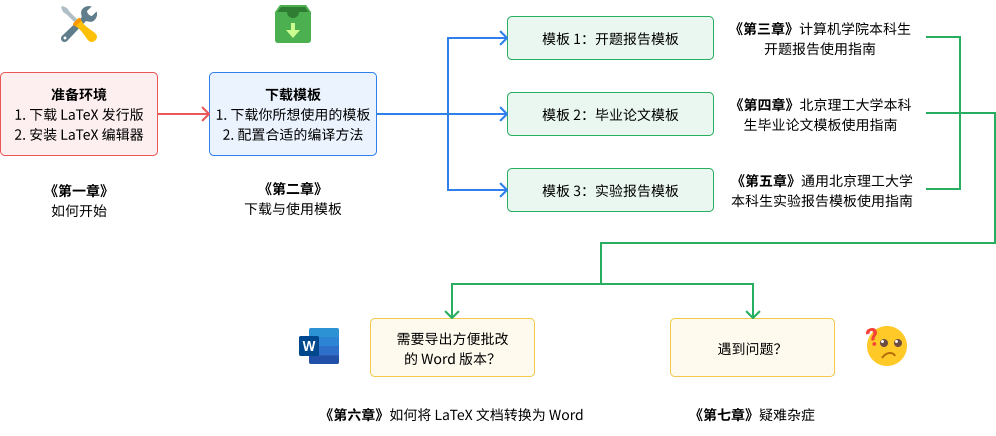
\includegraphics[width=\textwidth]{images/flowchart.png}
  \caption{使用本文档与 {\BIThesis} 的顺序}
  \label{flowchart}
\end{figure}

\subsection{在线说明文档:Wiki}
和本手册的目标类似,{\BIThesis} 项目同样维护了一个在线版本的说明文档,位于:{\href{https://bithesis.spencerwoo.com/}{BIThesis - wiki}},二者的目的、内容、功能类似,且会随着模板的开发与维护同步更新。

{\BIThesis} 在线说明文档目前拥有与本手册一致的如下模块:

\begin{enumerate}
  \item \href{https://bithesis.spencerwoo.com/Guide/}{主页:Home}
  \item \href{https://bithesis.spencerwoo.com/Guide/1-Intro/First-things-first}{如何开始:First things first }
  \item \href{https://bithesis.spencerwoo.com/Guide/2-Usage/Downloading-and-using-templates}{使用其中一个模板:Using one of the templates}
  \item \href{https://bithesis.spencerwoo.com/Guide/3-Templates/Proposal-Report}{本科生开题报告:Proposal report}
  \item \href{https://bithesis.spencerwoo.com/Guide/3-Templates/Final-Graduation-Thesis}{本科生毕业论文:Graduation thesis}
  \item \href{https://bithesis.spencerwoo.com/Guide/3-Templates/Lab-Report}{本科生实验报告:Lab report}
  \item \href{https://bithesis.spencerwoo.com/Guide/4-Others/Converting-to-Word}{将 LaTeX 文档转换为 Word:Converting to Word}
  \item \href{https://bithesis.spencerwoo.com/Guide/4-Others/Troubleshooting}{疑难杂症:Troubleshooting}
\end{enumerate}

接下来,我们正式开始介绍 {\LaTeX} 与 {\BIThesis} 的使用方法。

\subsection{准备工作}
首先,在使用模板之前,你需要在本机安装 \LaTeX 环境。一个完整的 \LaTeX 环境包括:

\begin{itemize}
  \item 开源免费的 \LaTeX 发行版(包含有必备的 \LaTeX 编译器与有用的宏包)
  \item 以及一个得心应手的 \LaTeX 编辑器
\end{itemize}

我们在 Windows、macOS 与 Linux 环境中均可以使用 \LaTeX 进行文档撰写。按照操作系统的不同,我们分别进行介绍。

\subsection{下载合适的 \LaTeX 发行版}
\importantbox{\textbf{注意:}{\BIThesis} 中参考文献为了和校方规定的模板格式《信息与文献参考文献著录规则》(\href{http://openstd.samr.gov.cn/bzgk/gb/newGbInfo?hcno=7FA63E9BBA56E60471AEDAEBDE44B14C}{GB/T 7714—2015})保持一致,使用了仅支持 \TeX Live 2019 版本的宏包,如果你曾经安装过 \TeX Live 且目前正在使用的 \TeX Live 版本不是 2019 版本,那么请及时更新为最新的 \TeX Live 2019 版本。}

\subsubsection{Windows 和 Linux 系统}
对于 Windows 和 Linux 系统,我们可以直接下载使用 \href{https://www.tug.org/texlive/}{\TeX Live 发行版}。

\paragraph{在线安装} 官方的安装指南位于:\href{https://www.tug.org/texlive/acquire-netinstall.html}{Installing \TeX Live over the Internet}。使用这一方法会下载 \texttt{install-tl-windows.exe}(Windows)或 \texttt{install-tl-unx.tar.gz}(Linux),之后运行相应的可执行程序,安装程序即可将整个 \TeX Live 发行版下载安装到我们本机。(通常会安装 3GB 左右的程序。)

\begin{figure}[H]
  \centering
  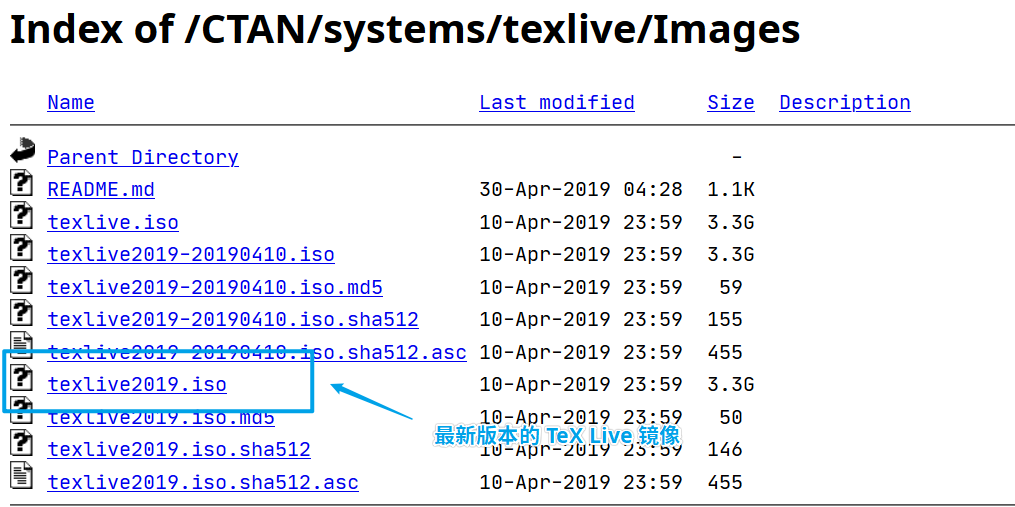
\includegraphics[width=\textwidth]{images/bit_mirror_texlive.png}
  \caption{北京理工大学开源镜像站 \TeX Live 下载}
  \label{mirrorbit}
\end{figure}

\paragraph{离线安装} 使用北京理工大学校园网的同学也可以直接使用我校官方 \TeX Live 镜像进行安装。我校 \TeX Live 镜像资源位于 \href{https://mirrors.bit.edu.cn/CTAN/systems/texlive/Images}{/CTAN/systems/texlive/Images},其中我们选择下载 \texttt{texlive2019.iso} 即可,如图 \ref{mirrorbit} 所示。Windows 10 可直接挂载 ISO 镜像(双击即可),其余系统用合适的软件也可。之后在打开的文件夹中点击执行 \texttt{install-tl-windows}(Windows)或 \texttt{install-tl}(Linux)即可离线安装全部 \TeX Live 组件。

\paragraph{使用包管理工具进行安装} 使用 Linux 系统的同学也可以选择使用合适的包管理工具进行 \TeX Live 的安装。以 Ubuntu 为例子,只需要运行下面命令,即可下载安装整个 \TeX Live 发行版。

\begin{minted}[frame=single]{bash}
  sudo apt install texlive
\end{minted}

\subsubsection{macOS 系统}
对于 macOS 系统,我们可以直接下载使用 \href{https://www.tug.org/mactex/}{Mac\TeX 发行版}。Mac\TeX 发行版是以 pkg 文件进行发布安装的,我们进入 \href{https://www.tug.org/mactex/mactex-download.html}{Max\TeX 的下载页面},点击下载 \texttt{MacTeX.pkg} 即可下载完整的 Mac\TeX 安装包(大约 3.9GB)。之后双击运行即可安装。

另外,使用 Homebrew 包管理的同学,也可以通过 Homebrew Cask 直接安装 Mac\TeX:

\begin{minted}[frame=single]{bash}
  # 加载 Homebrew Cask
  brew tap caskroom/cask

  # 利用 Cask 安装 MacTeX
  brew cask install mactex
\end{minted}

\subsubsection{确认安装}
为了保证我们 \LaTeX 发行版的安装没有问题,我们需要验证一下 \LaTeX 编译工具的安装情况。我们打开终端(Windows 打开 PowerShell、macOS 打开 Terminal、Linux 打开你所使用的终端模拟器),在其中输入下面的命令:

\begin{itemize}
  \item 验证 \texttt{latexmk} 和 \texttt{xelatex} {\LaTeX} 编译器的安装情况:
        \begin{minted}[
    frame=single
  ]{bash}
  # 验证 latexmk 的安装
  latexmk --version
  # 验证 xelatex 的安装
  xelatex --version
  \end{minted}
        \begin{figure}[H]
          \flushright
          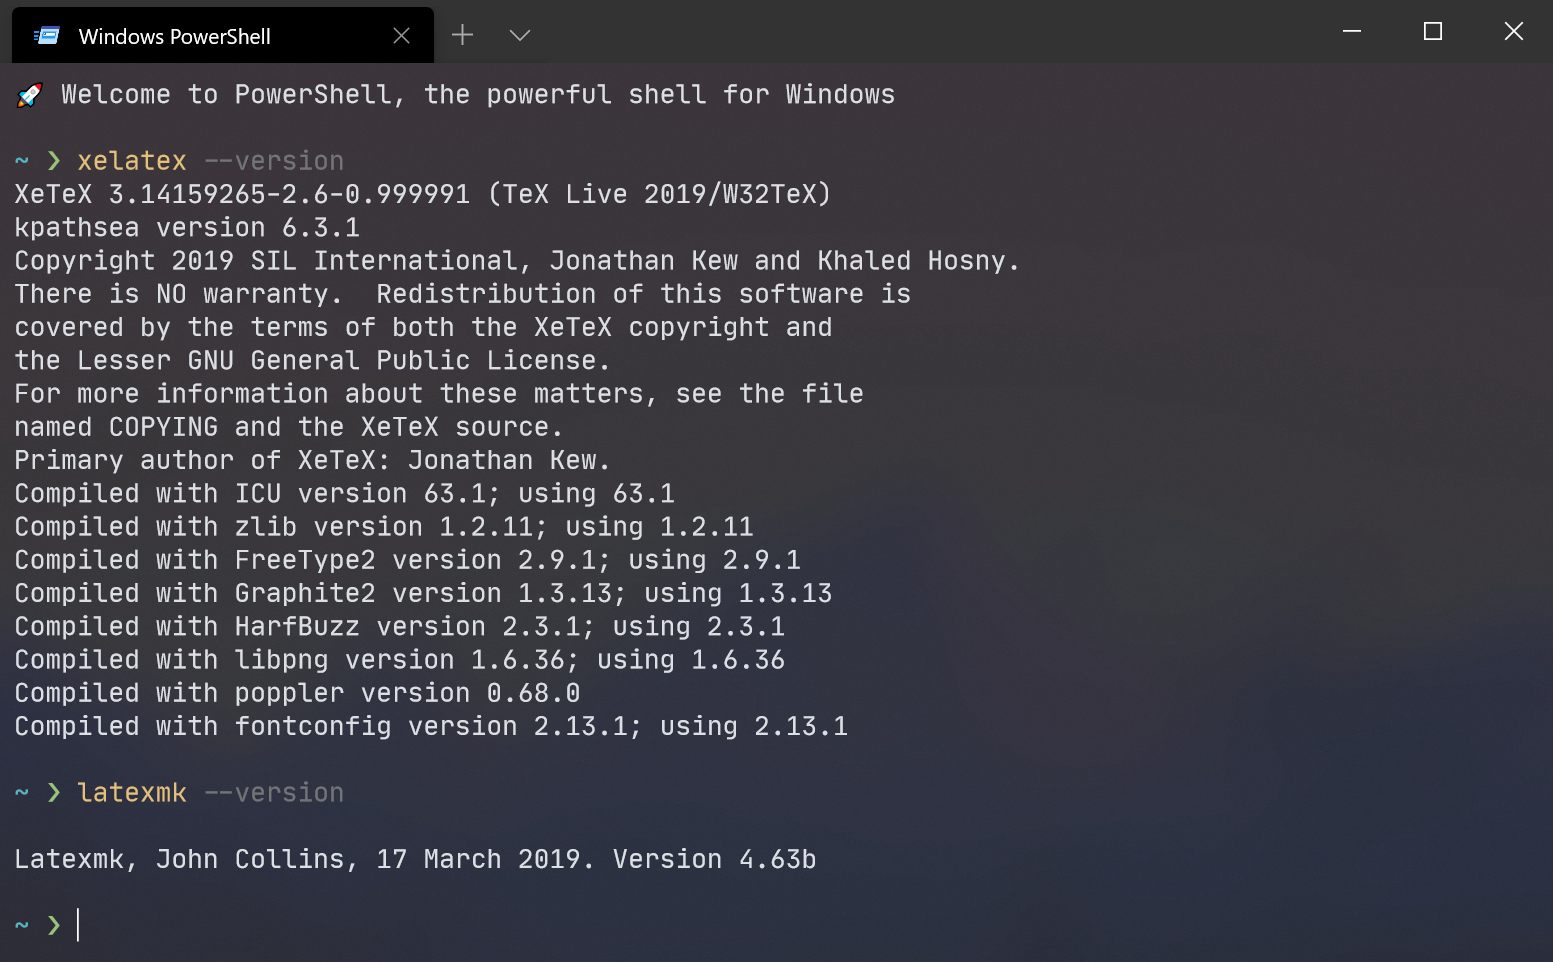
\includegraphics[width=0.93\textwidth]{images/xelatex.png}
          \caption{\hologo{XeLaTeX} 安装成功输出}
          \label{xelatex}
        \end{figure}
  \item 验证 \texttt{biber} 参考文献编译器的安装情况:
        \begin{minted}[
    frame=single
  ]{bash}
  biber --version
  \end{minted}
        \begin{figure}[H]
          \flushright
          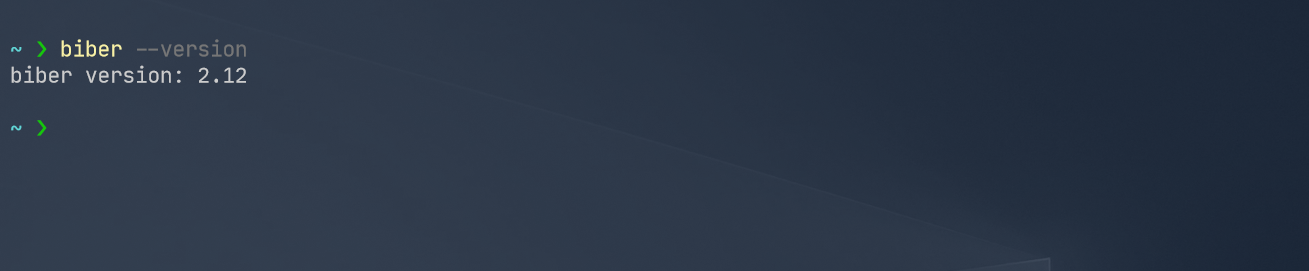
\includegraphics[width=0.93\textwidth]{images/biber.png}
          \caption{\hologo{biber} 安装成功输出}
          \label{biber}
        \end{figure}
\end{itemize}

出现如图 \ref{xelatex} 与 \ref{biber} 类似的输出,说明我们编译器安装应该是没有问题的。

\subsection{挑选合适的 \LaTeX 编辑器}
理论上来说,任何一个“文本编辑器”均可以用来撰写 {\LaTeX} 文档,但是一个得心应手的 {\LaTeX} 编辑器一定会让我们撰写论文的效率大增。

\subsubsection{使用 VS Code 配合 {\LaTeX} Workshop 插件编辑 \LaTeX 文档}
VS Code 是微软开发的基于 Electron 跨平台技术的新晋代码编辑器,开源免费、拓展性强、功能强大,是当代开发者的首选。用 VS Code 配合 {\LaTeX} Workshop 插件我们可以打造一个强大的 {\LaTeX} 编辑器。

\begin{figure}[H]
  \centering
  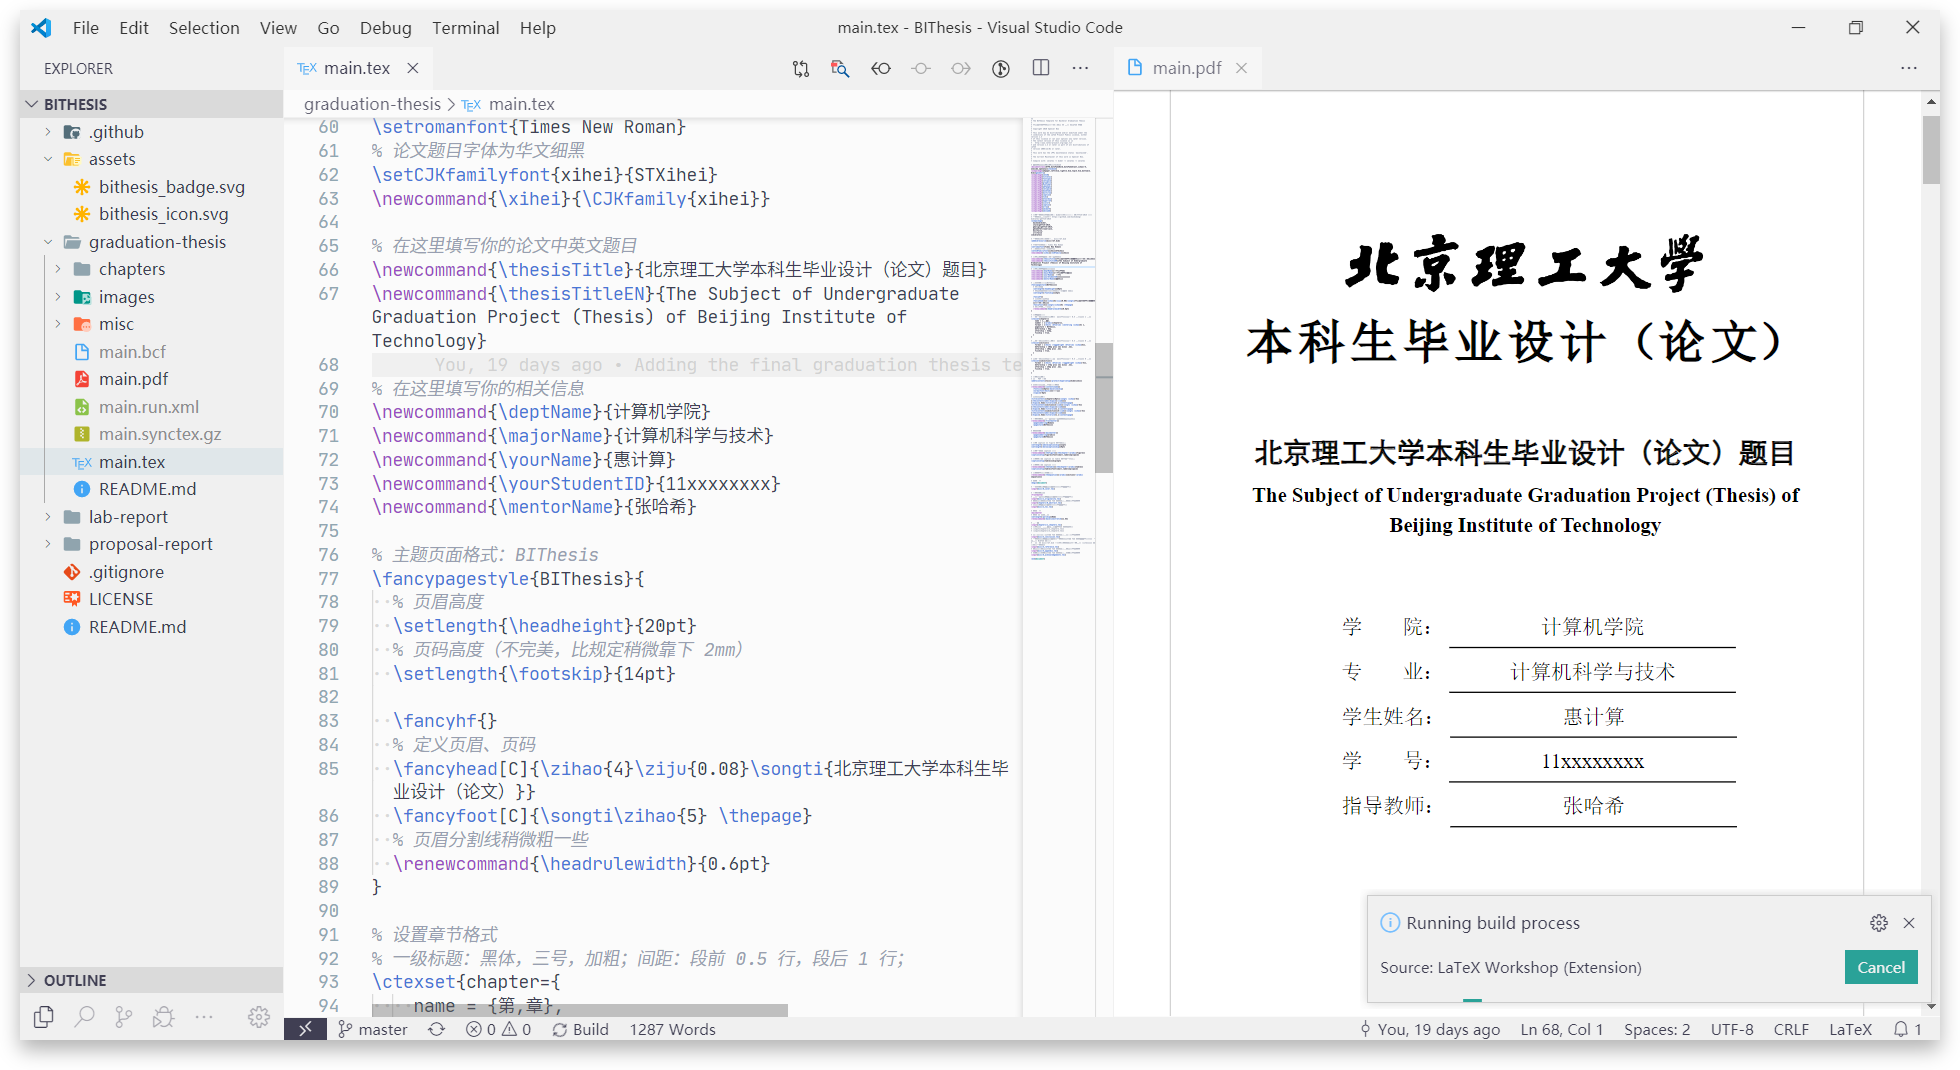
\includegraphics[width=\textwidth]{images/vscode.png}
  \caption{VS Code 代码编辑器}
\end{figure}

\begin{itemize}
  \item 安装 VS Code 编辑器:\href{https://code.visualstudio.com/}{Visual Studio Code - Code editing. Redefined.}
  \item 安装插件:
        \begin{itemize}
          \item 安装 {\LaTeX} Workshop 插件:\href{https://marketplace.visualstudio.com/items?itemName=James-Yu.latex-workshop}{Visual Studio Code LaTeX Workshop Extension}
                \begin{itemize}
                  \item 提供基本的浏览、编辑、自动补全、自动格式化 {\LaTeX} 文档的功能
                  \item 提供在 VS Code 内直接预览 {\LaTeX} 文档编译得到的 PDF 的功能
                  \item 提供编译工具链、自定义编译方法等功能
                        提供 SyncTeX 双向定位功能({\LaTeX} 源码 $\longleftrightarrow$ PDF)

                \end{itemize}
          \item (可选)安装 {\LaTeX} Utilities 插件:\href{https://marketplace.visualstudio.com/items?itemName=tecosaur.latex-utilities}{Visual Studio Code LaTeX Utilities}
                \begin{itemize}
                  \item 提供实时 {\LaTeX} 文档字数统计的功能
                  \item 提供与参考文献管理工具 Zotero 连接的功能
                \end{itemize}
        \end{itemize}
\end{itemize}

使用 VS Code 作为 {\LaTeX} 编辑器时,我们需要特别配置编译工具 \texttt{tools} 与编译工具链 \texttt{recipes}。对于包含有目录、参考文献、图片与表格引用的 {\LaTeX} 文档,我们往往需要使用多个编译工具串联编译。具体的 VS Code 编译方法,请继续阅读下一章《第 \ref{sec:downloading-templates} 章:下载与使用模板》。

\subsubsection{使用 \TeX studio 编辑 \LaTeX 文档}
\importantbox{注意:使用 macOS 的同学,请谨慎使用 \TeX studio,据反映 \TeX studio 有比较复杂难以解决的问题,因此请使用 Mac 的同学尽量使用 VS Code(或下文提到的付费 Texpad)来使用本模板。}

\TeX studio 是老牌 {\LaTeX} 编辑器,使用跨平台技术 Qt 编写而成。虽然界面相对老旧,但是依旧可靠。我们可以去 \href{https://www.texstudio.org/}{\TeX studio 的官网}下载安装各个系统版本的 \TeX studio。

\begin{figure}[H]
  \centering
  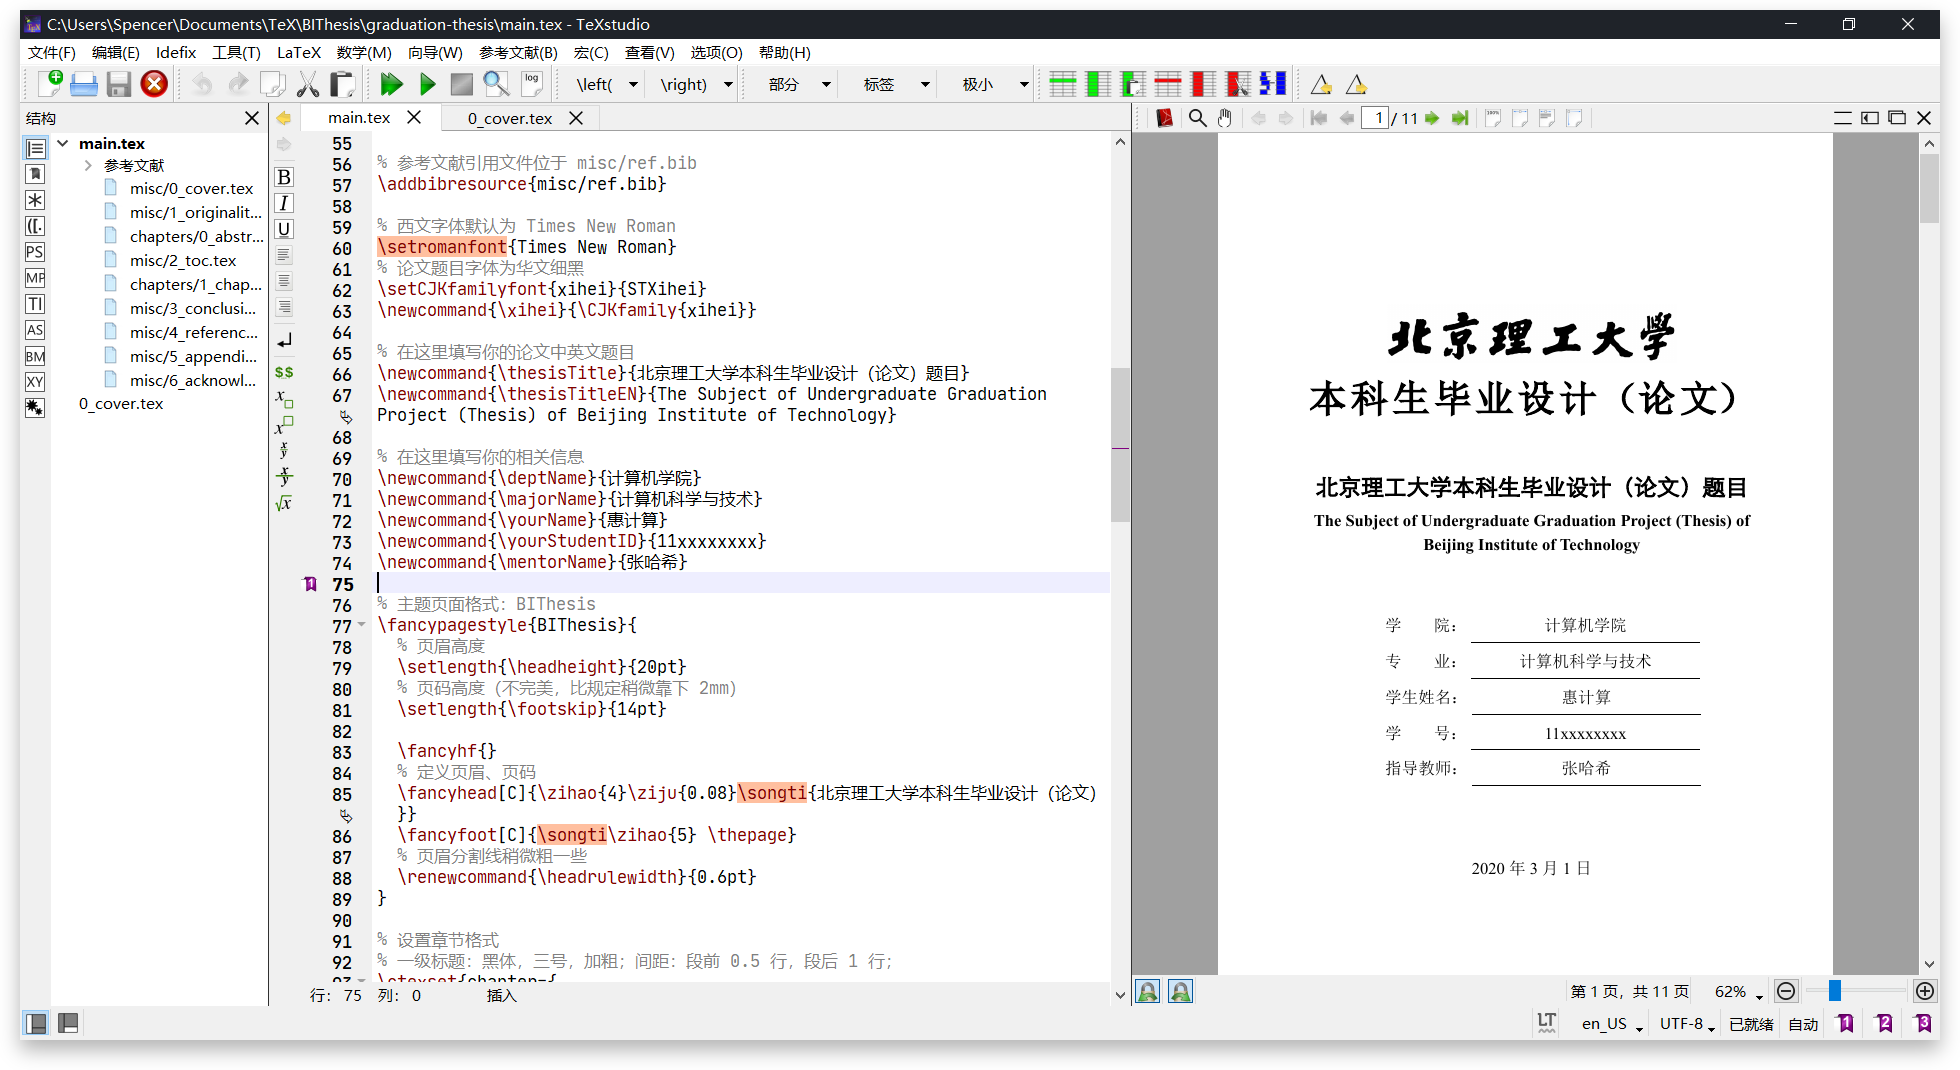
\includegraphics[width=\textwidth]{images/texstudio.png}
  \caption{\TeX studio 老牌 {\LaTeX} 编辑器}
\end{figure}

默认情况下 \TeX studio 的编译工具链均已经配置完毕,基本开箱即用。对于如何用 \TeX studio 编译本模板,请继续阅读下一章《第 \ref{sec:downloading-templates} 章:下载与使用模板》。

\tipbox{另外,如果你是特别不差钱的 Mac 用户,希望用最好用最牛逼的 {\LaTeX} 编辑器,你也可以去购买目前售价 \$29.99 美元(约合人民币 209.69 元)的 Texpad。使用 macOS、iOS 原生技术栈开发,Texpad 可能是目前使用体验最顺滑的 {\LaTeX} 编辑器,另外由于 Texpad 使用私有 {\LaTeX} 发行版,使得 Texpad 支持实时预览成果 PDF 与双向同步滚动支持。有这方面需要(与金钱)的同学可以考虑入手。}

准备就绪后,我们就可以开始使用 {\BIThesis} 提供的模板进行 {\LaTeX} 文档的撰写啦!

\clearpage
\section{下载与使用模板} \label{sec:downloading-templates}
{\BIThesis} 整个项目中包含多个模板,每个模板各自位于独立的文件夹中。

\subsection{熟悉简单 \LaTeX 语法} \label{subsec:latex-grammar}
如果你之前没有接触过 {\LaTeX},请前往 Overleaf 的“\href{https://www.overleaf.com/learn/latex/Learn_LaTeX_in_30_minutes}{30 分钟学习 {\LaTeX}}”文档进行阅读,从而对 {\LaTeX} 有大致的印象。

一些常用的 {\LaTeX} 格式与使用技巧:

\begin{itemize}
  \item \href{https://www.overleaf.com/learn/latex/Sections_and_chapters}{{\LaTeX} 章节设定:Sections and chapters}
  \item \href{https://www.overleaf.com/learn/latex/Paragraphs_and_new_lines}{{\LaTeX} 段落格式:Paragraphs and new lines}
  \item \href{https://www.overleaf.com/learn/latex/Bold,_italics_and_underlining}{{\LaTeX} 粗体、斜体与下划线:Bold, italics and underlining}
  \item \href{https://www.overleaf.com/learn/latex/Lists}{{\LaTeX} 有序列表、无序列表:Lists}
  \item \href{https://www.overleaf.com/learn/latex/Inserting_Images}{{\LaTeX} 插入图片:Inserting Images}
  \item \href{https://www.overleaf.com/learn/latex/Tables}{{\LaTeX} 构建表格:Tables}
  \item \href{https://www.overleaf.com/learn/latex/Mathematical_expressions}{{\LaTeX} 插入数学公式:Mathematical expressions}
  \item \href{https://www.overleaf.com/learn/latex/Code_Highlighting_with_minted}{{\LaTeX} 插入代码与代码高亮:Code Highlighting with minted}
  \item \href{https://www.overleaf.com/learn/latex/algorithms}{{\LaTeX} 插入算法伪代码描述:Algorithms}
  \item \href{https://www.overleaf.com/learn/latex/Bibliography_management_in_LaTeX}{使用 {Bib\LaTeX} 管理参考文献:Bibliography management in LaTeX}
\end{itemize}

有关 {\LaTeX} 使用的更多技巧,请直接前往 \href{https://www.overleaf.com/learn/latex/Main_Page}{Overleaf 官方文档}进行查看。准备就绪之后,你就可以前往下载 {\BIThesis} 模板啦。

\subsection{在项目的 Release 页面下载你希望使用的模板}
为了方便各位同学使用,项目按照 Release 发布的流程,将每个模板进行打包,并在每次发版后用 GitHub Release 进行模板分发。也就是,你可以直接前本项目的 GitHub Release 页面,直接下载你所希望使用的模板压缩包,并解压到本地进行使用。

你可以点击这个链接前往最新的 Release 版本进行模板下载:

\begin{center}
  \color{ForestGreen}\href{https://github.com/spencerwooo/BIThesis/releases/latest}{https://github.com/spencerwooo/BIThesis/releases/latest}
\end{center}

在 Release 页面,你会看到:

\dirtree{%
.1 /.
.2 proposal-report.zip \ldots{} \color{RoyalBlue}{本科生毕业设计开题报告模板压缩包}.
.2 graduation-thesis.zip \ldots{} \color{RoyalBlue}{本科生毕业设计毕业论文模板压缩包}.
.2 lab-report.zip \ldots{} \color{RoyalBlue}{本科生实验报告模板压缩包}.
}

\begin{figure}[H]
  \centering
  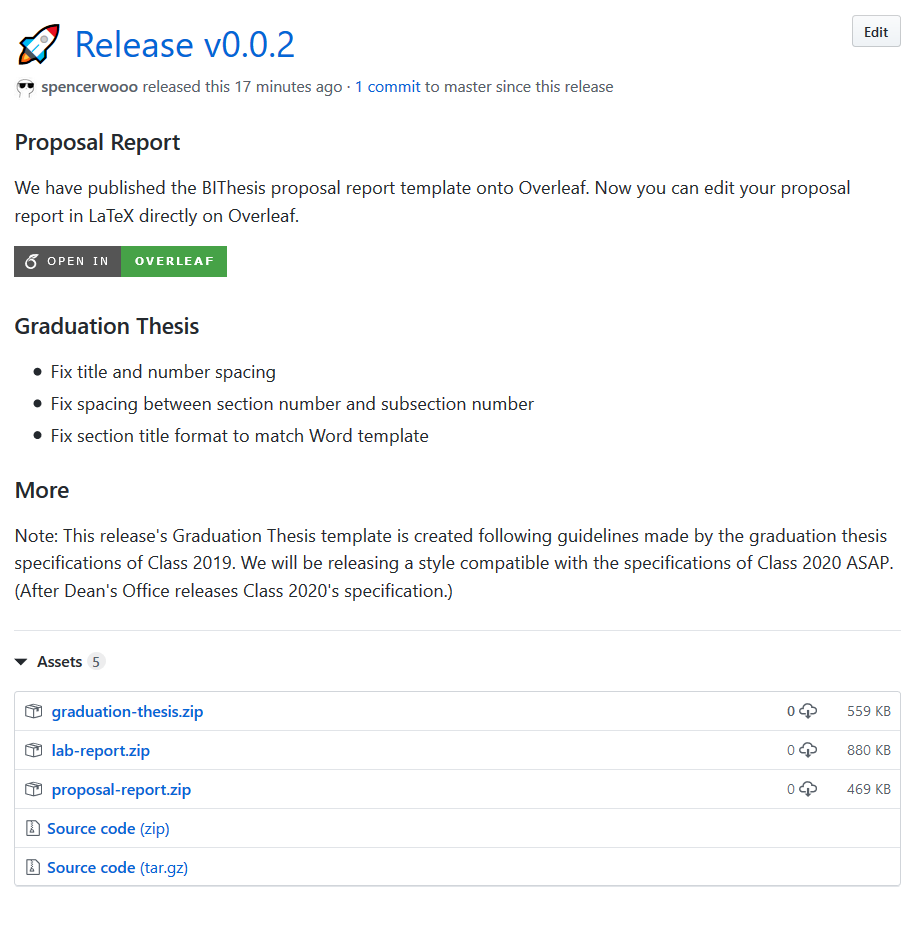
\includegraphics[width=\textwidth]{images/release.png}
  \caption{{\BIThesis} 的 Release 页面}
\end{figure}

根据你的选择,下载其中你所要使用的模板即可。(当然,你也可以直接用 Git 将本项目完整克隆至本地,使用最新版本的模板。)

\subsection{编译模板}

与 Word 不同的是,{\LaTeX} 模板需要我们用合适的工具进行编译,才能生成最终 PDF 文件。我们接下来介绍 {\BIThesis} 中的模板在各个编辑器中的编译方法。

{\BIThesis} 中的模板编译方式大同小异,我们都会使用 \hologo{XeLaTeX}、\hologo{biber} 以及 \texttt{latexmk} 等工具来编译它们。编译 {\BIThesis} 有两种方法:

\begin{enumerate}
  \item 使用 \texttt{xelatex} 配合 \texttt{biber} 进行编译:需要使用“四步走” \texttt{xelatex -> biber -> xelatex -> xelatex} 的编译顺序编译模板,全量编译,编译一次可能花费较长时间
  \item 使用 \texttt{latexmk} 进行编译:只需要使用一次 \texttt{latexmk} 即可编译整个模板,自动识别参考文献编译器,增量编译
\end{enumerate}

这两种编译方式均可以用于编译我们的模板,大家可以综合自己的使用习惯来挑选工具。事实上,后面我们将要介绍的 {\LaTeX} 编辑器,它们背后所使用的编译方法就是运行这里提到的两种编译工具。只是我们需要单独配置编辑器的编译方法,才能让编辑器正确的调用编译方式,编译我们的 {\LaTeX} 文档。

在这里,我挑选了三种常见的 {\LaTeX} 编写环境:

\begin{itemize}
  \item 直接使用“命令行”徒手编写编译
  \item 使用 VS Code 配合 {\LaTeX} Workshop 编写与编译
  \item 使用 \TeX studio 编写与编译
\end{itemize}

我会依次介绍在这三种环境下 {\LaTeX} 编译器配置方法。

\subsubsection{徒手编译}

当然,你完全可以不借助任何编辑器,直接使用“命令行”编译 {\LaTeX} 文档。

\paragraph{使用 \hologo{XeLaTeX} 编译}

如果你使用 \hologo{XeLaTeX} 编译项目,那么你需要按照下面的顺序依次调用 \texttt{xelatex} 与 \texttt{biber} 命令行工具:

\begin{center}
  \begin{tikzpicture}[
    bib/.style={rectangle, draw=ForestGreen!60, fill=ForestGreen!5, very thick, minimum size=8mm},
    xe/.style={rectangle, draw=RubineRed!60, fill=RubineRed!5, very thick, minimum size=8mm},
    ]
  % Nodes
  \node[xe] (xelatex1) {xelatex};
  \node[bib] (biber) [right=of xelatex1] {biber};
  \node[xe] (xelatex2) [right=of biber] {xelatex};
  \node[xe] (xelatex3) [right=of xelatex2] {xelatex};

  % Arrows
  \draw[->] (xelatex1.east) -- (biber.west);
  \draw[->] (biber.east) -- (xelatex2.west);
  \draw[->] (xelatex2.east) -- (xelatex3.west);
  \end{tikzpicture}
\end{center}

比如,编译主文档为 \texttt{main.tex} 的 {\LaTeX} 项目,我们具体的命令为:

\begin{minted}[frame=single,linenos,breaklines]{bash}
  # 第一步 xelatex
  xelatex -no-pdf --interaction=nonstopmode main
  # 第二步 biber
  biber main
  # 第三步 xelatex
  xelatex -no-pdf --interaction=nonstopmode main
  # 第四步 xelatex
  xelatex --interaction=nonstopmode main
\end{minted}

\paragraph{使用 \texttt{latexmk} 编译}

如果你使用 \texttt{latexmk} 编译模板,那么你只需要使用如下的命令即可编译主文件为 \texttt{main.tex} 的 {\LaTeX} 项目:

\begin{minted}[frame=single,linenos,breaklines]{bash}
  # 只需要调用一次 latexmk 工具即可
  latexmk -synctex=1 -interaction=nonstopmode -file-line-error -xelatex main.tex
\end{minted}

\subsubsection{使用 VS Code 撰写与编译 {\LaTeX} 模板}

VS Code 的设置项目可以通过快捷键 \keys{\ctrl \  or\ \cmd + ,})打开 UI 设置界面,之后点击右上角 \texttt{Open Settings (JSON)} 按钮即可打开相应的 JSON 格式配置文件,我们在这里即可定义 {\LaTeX} 编译工具。其中:

\begin{itemize}
  \item “编译工具”是在 \texttt{"latex-workshop.latex.tools": [ ... ]} 处进行定义,即我们在这里定义每次调用工具 \texttt{xelatex} 或 \texttt{latexmk} 时所执行的命令
  \item “编译工具链”是在 \texttt{"latex-workshop.latex.recipes": [ ... ]} 处进行定义,即我们在这里定义编译整个文档的工具链。对我们的模板第一种编译方式来说,就是定义 \texttt{xelatex -> biber -> xelatex -> xelatex} “四步走”的串联过程
\end{itemize}

\paragraph{使用 \hologo{XeLaTeX} 编译}
这种方法需要调用的工具有:\texttt{xelatex} 和 \texttt{biber}。我们在 VS Code 的设置中加入如下内容定义这两个工具:

\begin{minted}[frame=single,linenos,breaklines]{json}
  "latex-workshop.latex.tools": [
    {
      "name": "xelatex",
      "command": "xelatex",
      "args": [
        "-synctex=1",
        "-interaction=nonstopmode",
        "-file-line-error",
        "-pdf",
        "-outdir=%OUTDIR%",
        "-cd",
        "%DOC%"
      ],
      "env": {}
    },
    {
      "name": "biber",
      "command": "biber",
      "args": [
          "%DOCFILE%"
      ],
      "env": {}
    }
  ]
\end{minted}

用这一方法编译整个文档的工具链串联方法是 \texttt{xelatex -> biber -> xelatex -> xelatex} “四步走”。我们在 VS Code 的设置中加入如下内容定义这个工具链:

\begin{minted}[frame=single,linenos,breaklines]{json}
  "latex-workshop.latex.recipes": [
    {
      "name": "xelatex -> biber -> xelatex * 2",
      "tools": [
        "xelatex",
        "biber",
        "xelatex",
        "xelatex"
      ]
    }
  ]
\end{minted}

\paragraph{使用 \texttt{latexmk} 编译}

这种方法我们只需要使用 \texttt{latexmk} 这一个命令行工具。我们在 VS Code 的设置中添加如下的内容定义这一工具:

\begin{minted}[frame=single,linenos,breaklines]{json}
  "latex-workshop.latex.tools": [
    {
      "name": "latexmk",
      "command": "latexmk",
      "args": [
        "-synctex=1",
        "-interaction=nonstopmode",
        "-file-line-error",
        "-xelatex",
        "-outdir=%OUTDIR%",
        "-cd",
        "%DOC%"
      ],
      "env": {}
    },
  ]
\end{minted}

之后我们再填入下面的内容定义整个工具链(只有一个 \texttt{latexmk}):

\begin{minted}[frame=single,linenos,breaklines]{json}
  "latex-workshop.latex.recipes": [
    {
      "name": "latexmk",
      "tools": [
        "latexmk"
      ]
    },
  ]
\end{minted}

之后,我们使用快捷键 \keys{\ctrl \  or\ \cmd + \shift + P} 打开命令执行栏,并搜索“LaTeX Workshop: Build with recipe”,并选择你所用的 recipe(即上面配置的工具链),即可编译整个 {\LaTeX} 项目。

\begin{figure}[H]
  \centering
  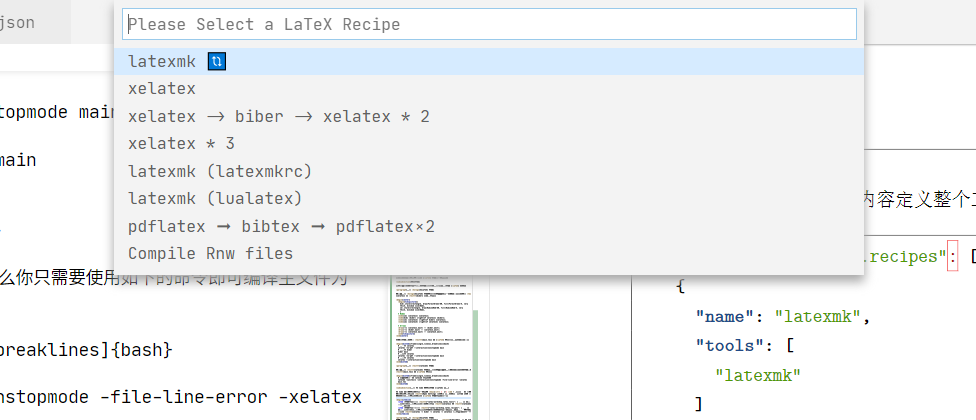
\includegraphics[width=\textwidth]{images/vscode_build_recipe.png}
  \caption{VS Code 挑选 recipe 工具链来编译 {\LaTeX} 项目}
\end{figure}

\subsubsection{使用 \TeX studio 撰写与编译 {\LaTeX} 模板}

\TeX studio 的编译工具大部分已经为我们配置完毕,我们只需要在 \TeX studio 的设置中定义编译所用的编译器即可。在 \TeX studio 中点击“选项 » 设置 TeXstudio”,在打开的窗口中选择“构建”,并在元命令里面将“默认编译器”设置为 \texttt{xelatex} 或 \texttt{latexmk},将默认文献工具设置为 \texttt{biber} 即可。

\begin{figure}[H]
  \centering
  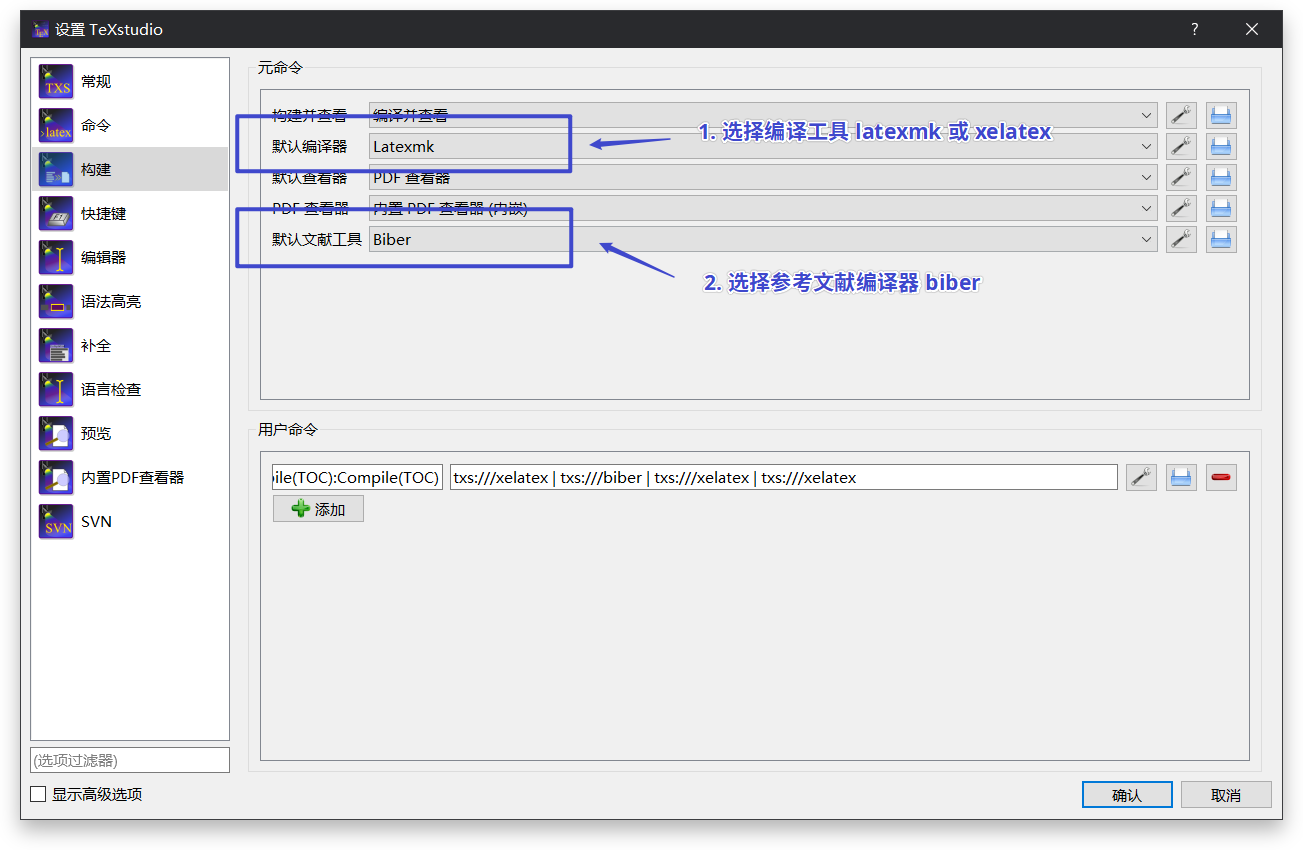
\includegraphics[width=\textwidth]{images/texstudio_build.png}
  \caption{\TeX studio 挑选默认编译器和参考文献工具来编译 {\LaTeX} 项目}
\end{figure}

你可以使用快捷键 \keys{F5} 一键编译与预览 {\LaTeX} 项目。

接下来,请继续在《第 \ref{proposal} 章》、《第 \ref{grad-thesis} 章》和《第 \ref{lab-report} 章》中阅读各个模板的详细模块介绍与用模板撰写论文的具体实施方法。

\clearpage
\section{计算机学院本科生开题报告使用指南} \label{proposal}

本模板已经发布在 Overleaf 上,你可以打开直接使用(点击下图 \ref{overleaf-proposal} 所示中的 Open as Template 即可:

\begin{center}
  \color{ForestGreen}\href{https://www.overleaf.com/latex/templates/bei-jing-li-gong-da-xue-ben-ke-sheng-bi-ye-lun-wen-kai-ti-bao-gao-mo-ban/dgqdjptfqtrn}{https://www.overleaf.com/latex/templates/bei-jing-li-gong-da-xue-ben-ke-sheng-bi-ye-lun-wen-kai-ti-bao-gao-mo-ban/dgqdjptfqtrn}
\end{center}

\begin{figure}[H]
  \centering
  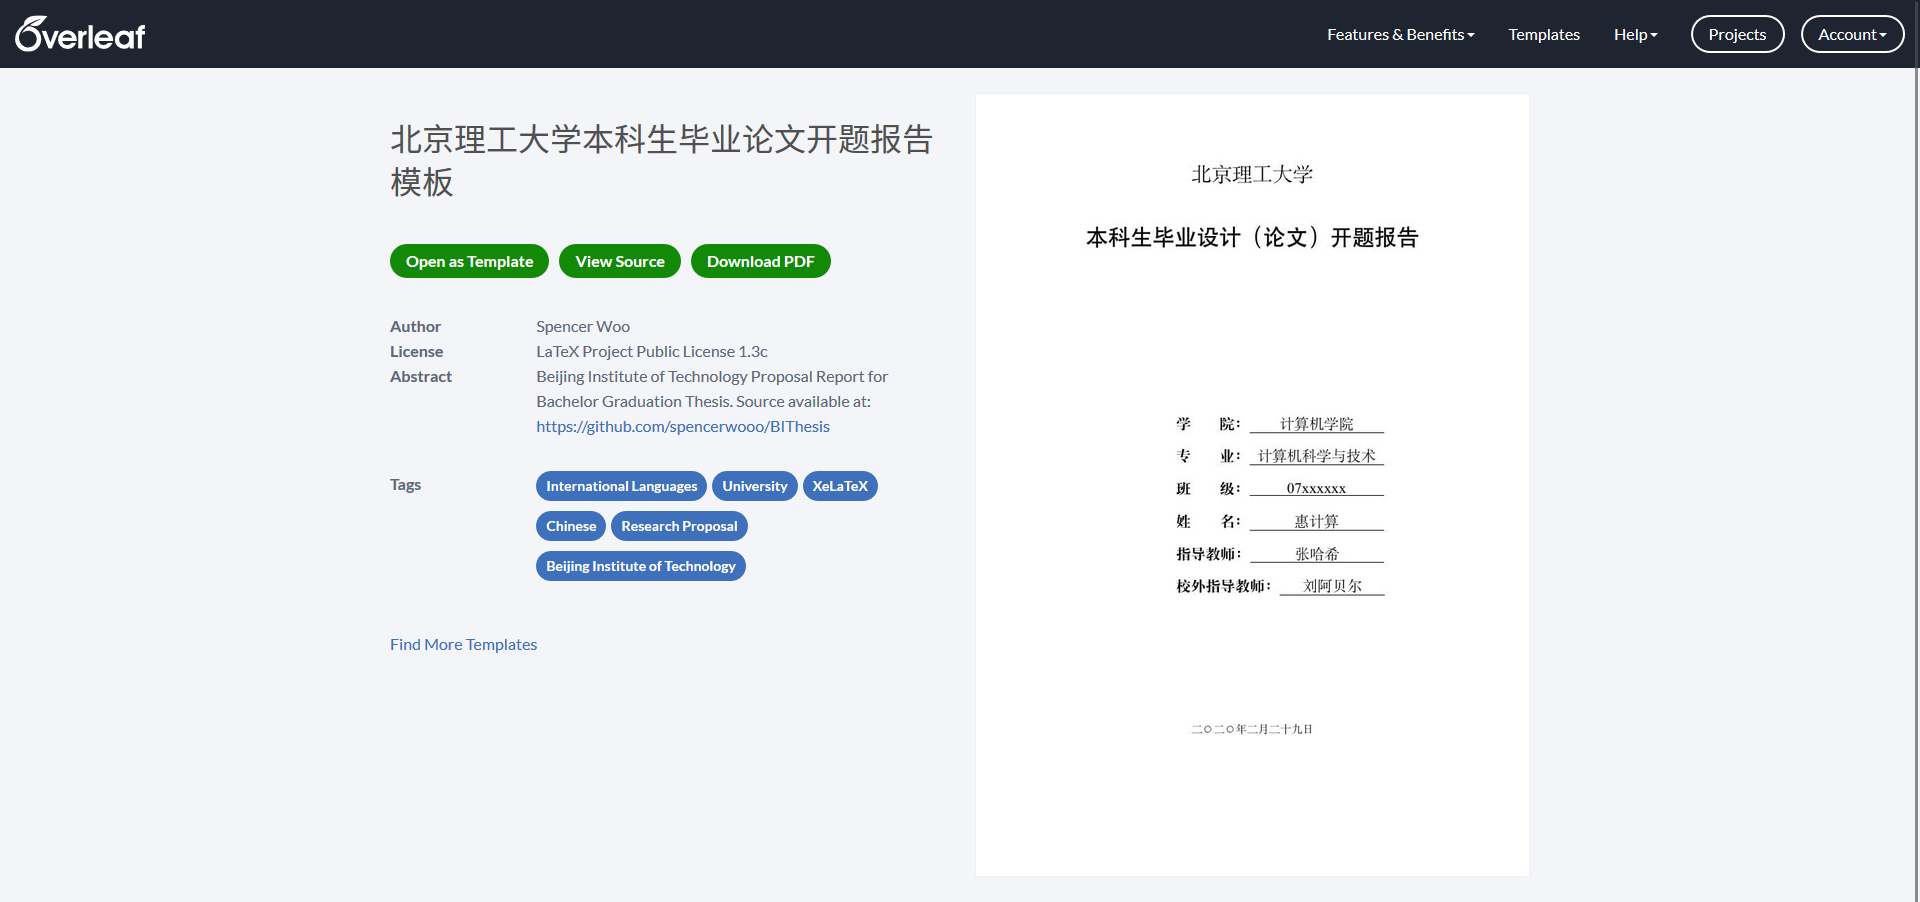
\includegraphics[width=\textwidth]{images/overleaf.png}
  \caption{Overleaf 在线版本的开题报告模板}
  \label{overleaf-proposal}
\end{figure}

Overleaf 缺少一些微软版权字体(比如宋体、黑体等),\textbf{因此如果你希望格式完全准确,请使用本机进行编辑。}

\subsection{熟悉项目}
% 输出文件数,第一行百分号 % 不能删,详见:http://tug.ctan.org/macros/generic/dirtree/dirtree.pdf
\dirtree{%
.1 /.
.2 README.md.
.2 main.pdf.
.2 main.tex.
.2 merge-sort-recursion-tree.png.
.2 misc.
.3 cover.tex.
.3 refs.bib.
.3 reviewTableBlank.pdf.
}

本项目由四个主要文件编译而成:\texttt{main.tex}、\texttt{cover.tex}、\texttt{refs.bib} 与\\ \texttt{reviewTableBlank.pdf}(也包括文档中所涉及到的图片等素材文件,比如:\\ \texttt{merge-sort-recursion-tree.png})。请大家重点关注这四个文件的功能与作用:

\begin{itemize}
  \item[\color{RubineRed}\textbf{\texttt{main.tex}}] 开题报告的开始文件(主文件),你的报告内容应该从此文件开始撰写。\texttt{main.tex} 中有详细的注释,介绍了每一部分内容都有什么作用,请仔细阅读后进行相应的修改、
  \item[\color{RubineRed}\textbf{\texttt{main.pdf}}] 开题报告编译得到的 PDF 文件
  \item[\color{RubineRed}\textbf{\texttt{./misc}}] 开题报告中所需要的杂项所在文件夹,其中包含有:
  \begin{itemize}
    \item[\color{RoyalBlue}\texttt{cover.tex}] 开题报告封面,按照教务部提供的封面设计,如无特殊需要请不要修改
    \item[\color{RoyalBlue}\texttt{reviewTableBlank.pdf}] 开题报告 PDF 格式的“评审表”,由于考虑到评审表后期由评委老师填写,因此本部分如无需要也无需改动
    \item[\color{RoyalBlue}\texttt{refs.bib}] 开题报告的参考文献 {\hologo{BibTeX}} 数据库,你应该向其中加入开题报告中所需要的所有参考文献的 {\hologo{BibTeX}} 格式引用(详见下文)
  \end{itemize}
\end{itemize}

\subsection{你的内容从哪里开始?}
开题报告项目结构相对来说比较简单,因此你只需要重点关注 \texttt{main.tex} 这一文件 —— 项目的主文件。你的内容应该从 \texttt{main.tex} 第 127 行 的 \texttt{\%内容开始} 开始。你需要重点关注的部分有:

\begin{table}[H]
\centering
\caption{开题报告内容概要}
\label{tab:proposalreport}
\resizebox{\textwidth}{!}{%
\begin{tabular}{@{}rll@{}}
\toprule
\textbf{文章部分} & \textbf{内容主旨}      & \textbf{对应 {\LaTeX} 模板 section}    \\ \midrule
第一部分 & 选题内容      & \texttt{\textbackslash{}section\{毕业设计(论文)\}}        \\ \midrule
第二部分 & 研究方案      & \texttt{\textbackslash{}section\{研究方案\}}            \\ \midrule
2-1  & 主要任务      & \texttt{\textbackslash{}subsection\{本选题的主要任务\}}     \\
2-2  & 技术方案      & \texttt{\textbackslash{}subsection\{技术方案的分析、选择\}}   \\
2-3  & 实施方案所需环境  & \texttt{\textbackslash{}subsection\{实施技术方案所需的条件\}}  \\
2-4  & 存在问题与技术关键 & \texttt{\textbackslash{}subsection\{存在的主要问题和技术关键\}} \\
2-5  & 预期研究目标    & \texttt{\textbackslash{}subsection\{预期能够达到的研究目标\}}  \\ \midrule
第三部分 & 课题计划进度表   & \texttt{\textbackslash{}section\{课题计划进度表\}}         \\ \bottomrule
\end{tabular}%
}
\end{table}

以及最后的“参考文献”。你应该将参考文献的 {\hologo{BibTeX}} 引用复制进入 \texttt{./misc/refs.bib},并在正文中用 \verb|\cite{}| 的方法进行引用。其中 {\hologo{BibTeX}} 格式的引用内容可以在谷歌学术中搜索文章直接复制得到,也可以考虑使用 Zotero 等文献管理工具批量生成。

\subsection{其他注意事项}
\tipbox{有关具体的 {\LaTeX} 语法,请参考前文中《第二章 \ref{subsec:latex-grammar}》给出的参考链接与学习文档。以下是模板中提供的一些示例性代码。}

\subsubsection{插入图片}
如果你希望加入图片,可以将图片直接放在根目录(比如此处的\\ \texttt{merge-sort-recursion-tree.png}),或者统一将图片安置在一个文件夹下,在正文里按照相对路径进行引用。模板中有一处插入图片的参考样例,位于 \texttt{main.tex} 的 \href{https://github.com/BITNP/BIThesis/blob/master/proposal-report/main.tex#L138}{第 138 行},可以进行参考。比如,我填入一个放在 \texttt{images/BIT\_Name.jpg} 处的图片:

\begin{minted}[frame=single,linenos,breaklines]{latex}
  \begin{figure}[!ht]
    \centering
    
\includegraphics[width=0.6\linewidth]{images/BIT_Name.jpg}
    \caption{北京理工大学(一张示意图)}
    \label{fig:BITName}
  \end{figure}
\end{minted}

这样就会渲染如图 \ref{fig:BITName} 的效果:

\begin{figure}[!ht]
  \centering
  
\includegraphics[width=0.6\linewidth]{images/BIT_Name.jpg}
  \caption{北京理工大学(一张示意图)}
  \label{fig:BITName}
\end{figure}

\subsubsection{插入表格}
如果你希望插入表格,可以统一使用 \href{https://www.tablesgenerator.com/}{LaTeX Tables Generator} 进行生成,再粘贴进入模板之中。模板中有两处表格的参考样例,分别位于 \href{https://github.com/BITNP/BIThesis/blob/master/proposal-report/main.tex#L151}{第 151 行} 和 \href{https://github.com/BITNP/BIThesis/blob/master/proposal-report/main.tex#L176}{第 176 行},可以进行参考。比如:

\begin{minted}[frame=single,linenos,breaklines]{latex}
  \begin{table}[!ht]
    \centering
    \caption{硬件、软件环境}
    \label{tab:soft-hardware}
    \begin{tabular}{@{}lcl@{}}
      \toprule
                                & 指标     & \multicolumn{1}{c}{版本参数} \\ \midrule
      \multirow{2}{*}{硬件环境} & CPU      & Intel i7-6500U               \\ \cmidrule(l){2-3}
                                & RAM      & 8 GB                         \\ \midrule
      \multirow{2}{*}{软件环境} & 操作系统 & \begin{tabular}[c]{@{}l@{}}Windows 10 Pro x86\_64\\  Ubuntu 18.04.3 LTS\end{tabular}    \\ \cmidrule(l){2-3}
                                & Python   & Python 3.7.6                 \\ \bottomrule
    \end{tabular}
  \end{table}
\end{minted}

渲染效果如表 \ref{tab:proposalreport} 所示:

\begin{table}[!ht]
  \centering
  \caption{硬件、软件环境}
  \label{tab:soft-hardware}
  \begin{tabular}{@{}lcl@{}}
    \toprule
                              & 指标     & \multicolumn{1}{c}{版本参数} \\ \midrule
    \multirow{2}{*}{硬件环境} & CPU      & Intel i7-6500U               \\ \cmidrule(l){2-3}
                              & RAM      & 8 GB                         \\ \midrule
    \multirow{2}{*}{软件环境} & 操作系统 & \begin{tabular}[c]{@{}l@{}}Windows 10 Pro x86\_64\\  Ubuntu 18.04.3 LTS\end{tabular}    \\ \cmidrule(l){2-3}
                              & Python   & Python 3.7.6                 \\ \bottomrule
  \end{tabular}
\end{table}

\clearpage
\section{北京理工大学本科生毕业设计论文模板使用指南}

\tipbox{注意:目前版本的毕业设计论文是按照北京理工大学计算机学院 2015 级毕业论文模板进行的设计与排版,如果 2016 级毕业论文模板有任何格式更新,我们会及时在这里更新。}

\subsection{熟悉项目}

\dirtree{%
  .1 /.
  .2 README.md.
  .2 main.tex.
  .2 main.pdf.
  .2 chapters.
  .3 0\_abstract.tex.
  .3 1\_chapter1.tex.
  .2 images.
  .3 bit\_logo.png.
  .3 header.png.
  .2 misc.
  .3 0\_cover.tex.
  .3 1\_originality.tex.
  .3 2\_toc.tex.
  .3 3\_conclusion.tex.
  .3 4\_reference.tex.
  .3 5\_appendix.tex.
  .3 6\_acknowledgements.tex.
  .3 ref.bib.
}

本项目由一个主文件和与之并存的几个辅助文件夹中的文件构成:

\begin{itemize}
  \item[\color{RubineRed}\textbf{\texttt{main.tex}}] 毕业论文模板的主文件
  \item[\color{RubineRed}\textbf{\texttt{./chapters}}] 文件夹:包含有整个毕业论文的“摘要”和正文的全部“章节”
  \begin{itemize}
    \item[\color{RoyalBlue}\texttt{0\_abstract.tex}] 毕业论文的“摘要”(中文摘要与英文摘要)
    \item[\color{RoyalBlue}\texttt{1\_chapter1.tex}] 毕业论文正文“第一章”(示例章节)
    \item[\color{RoyalBlue}\texttt{...}] (你可以继续添加第二章 \texttt{2\_chapter2.tex}、第三章 \texttt{3\_chapter3.tex}……,并在主文件 \texttt{main.tex} 中引用(详见下文)
  \end{itemize}
  \item[\color{RubineRed}\textbf{\texttt{./misc}}] 文件夹:包含有毕业论文模板中的封面、后置章节与参考文献
  \begin{itemize}
    \item[\color{RoyalBlue}\textbf{\texttt{0\_cover.tex}}] 毕业论文的“封面”,一般情况无需更改
    \item[\color{RoyalBlue}\textbf{\texttt{1\_originality.tex}}] 毕业论文的“原创性声明”,一般情况无需更改(签字和日期后期手动添加)
    \item[\color{RoyalBlue}\textbf{\texttt{2\_toc.tex}}] 毕业论文的“目录”,一般情况无需更改(由 {\LaTeX} 自动生成)
    \item[\color{RoyalBlue}\textbf{\texttt{3\_conclusion.tex}}] 毕业论文的“结论”,按照一般章节文件对待
    \item[\color{RoyalBlue}\textbf{\texttt{4\_reference.tex}}] 毕业论文的“参考文献”,一般情况无需更改(由 {\LaTeX} 根据你文档中的 \verb|\cite{}| 自动生成)
    \item[\color{RoyalBlue}\textbf{\texttt{5\_appendix.tex}}] 毕业论文的“附录”,按照一般章节文件对待
    \item[\color{RoyalBlue}\textbf{\texttt{6\_acknow...ments.tex}}] 毕业论文的“致谢”,按照一般章节文件对待
    \item[\color{RoyalBlue}\textbf{\texttt{ref.bib}}] 参考文献 \hologo{BibTeX} 数据库
  \end{itemize}
\end{itemize}

主文件与其余文件之间的引用关系大致如下图 \ref{grad_thesis_main_submodule} 所示:

\begin{figure}[H]
  \center
  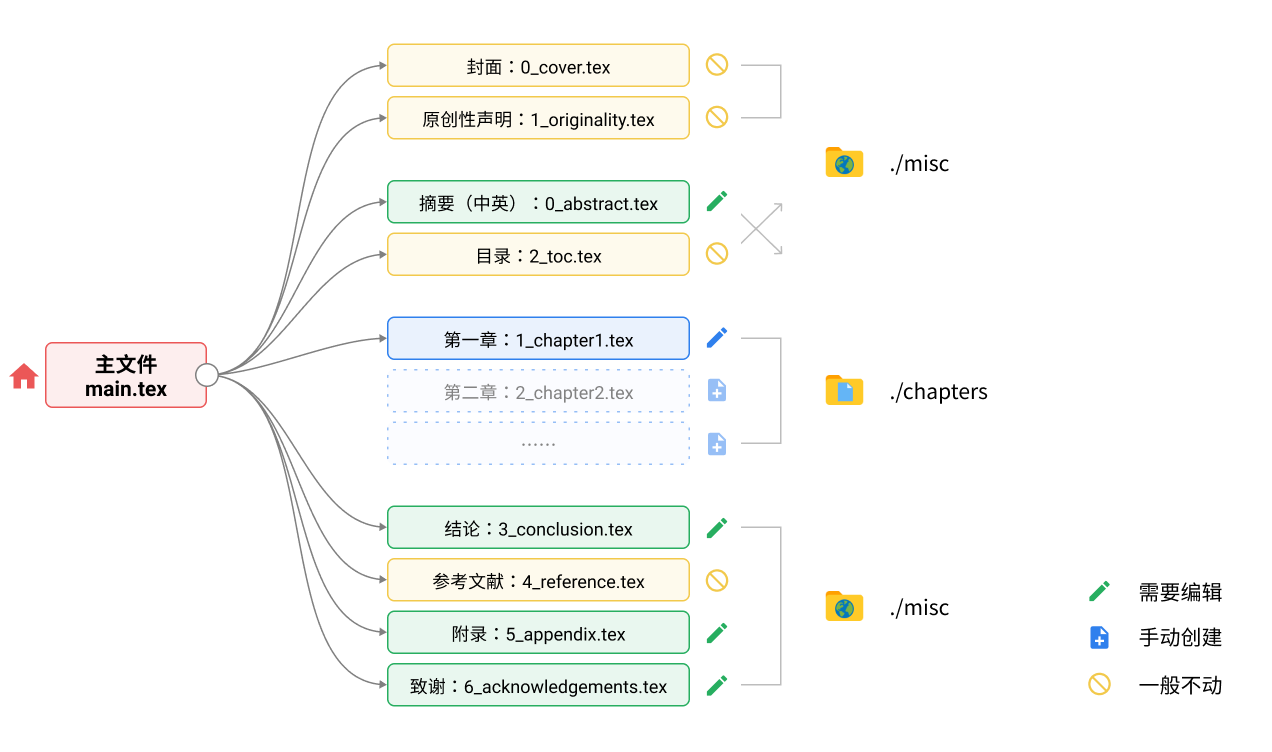
\includegraphics[width=\textwidth]{images/grad_thesis.png}
  \caption{毕业论文模板主模块与各个分支之间的关系}
  \label{grad_thesis_main_submodule}
\end{figure}

具体编译和使用,请见下文详细描述。

\subsection{使用与编译方式}

\subsubsection{使用 Overleaf 直接打开}

本模板已经发布在 Overleaf 上,你可以打开直接使用:

\begin{center}
  \color{ForestGreen}\href{https://www.overleaf.com/latex/templates/bei-jing-li-gong-da-xue-ben-ke-sheng-bi-ye-she-ji-lun-wen-mo-ban/mwhjgqsncxxg}{https://www.overleaf.com/latex/templates/bei-jing-li-gong-da-xue-ben-ke-sheng-bi-ye-she-ji-lun-wen-mo-ban/mwhjgqsncxxg}
\end{center}

\begin{figure}[H]
  \centering
  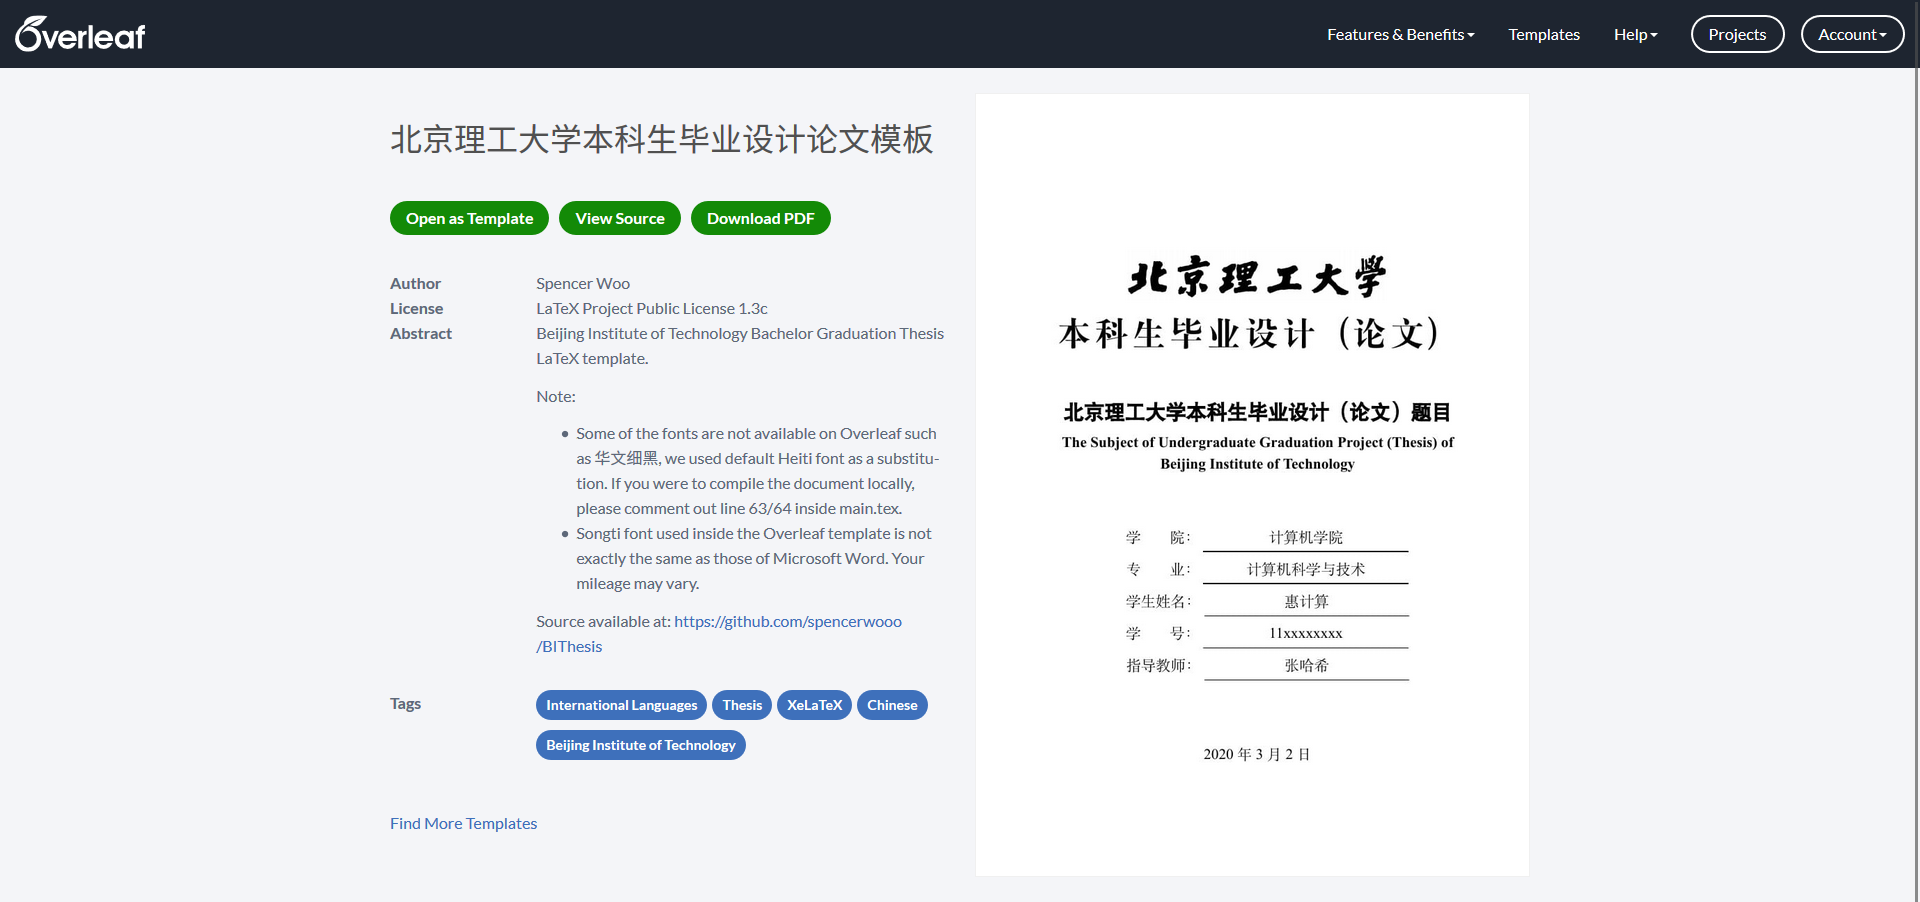
\includegraphics[width=\textwidth]{images/overleaf_grad_thesis.png}
  \caption{Overleaf 在线版本的毕业论文模板}
\end{figure}

Overleaf 版本的毕业论文模板中由于没有微软版权字体“华文细黑”,导致封面的毕业论文中文大标题无法用 Word 模板中规定的字体渲染,使得最终呈现样式与要求有些出入,如果希望保证 {\LaTeX} 模板输出和学校模板一致,那么还是推荐在本地进行撰写和编译。

\subsubsection{在本地撰写}

由于:

\begin{itemize}
  \item {\BIThesis} 文章主体部分是中文,使用了 \texttt{ctex} 宏包,因此需要使用 \texttt{xelatex} 进行全文编译
  \item 参考文献部分使用了 {Bib\LaTeX},因此需要使用 \hologo{biber} 进行参考文献的编译
\end{itemize}

\paragraph{使用 {\hologo{XeLaTeX}} 编译}
整个项目的编译工具链的顺序为:

\begin{center}
  \begin{tikzpicture}[
    bib/.style={rectangle, draw=ForestGreen!60, fill=ForestGreen!5, very thick, minimum size=8mm},
    xe/.style={rectangle, draw=RubineRed!60, fill=RubineRed!5, very thick, minimum size=8mm},
    ]
  % Nodes
  \node[xe] (xelatex1) {xelatex};
  \node[bib] (biber) [right=of xelatex1] {biber};
  \node[xe] (xelatex2) [right=of biber] {xelatex};
  \node[xe] (xelatex3) [right=of xelatex2] {xelatex};

  % Arrows
  \draw[->] (xelatex1.east) -- (biber.west);
  \draw[->] (biber.east) -- (xelatex2.west);
  \draw[->] (xelatex2.east) -- (xelatex3.west);
  \end{tikzpicture}
\end{center}


其中,按照 VS Code 的 LaTeX Workshop 设置格式:

\begin{itemize}
  \item {\hologo{XeLaTeX}} 的编译命令为:
  \begin{minted}[frame=single]{json}
  {
    "name": "xelatex",
    "command": "xelatex",
    "args": [
      "-synctex=1",
      "-interaction=nonstopmode",
      "-file-line-error",
      "-pdf",
      "-outdir=%OUTDIR%",
      "-cd",
      "%DOC%"
    ],
    "env": {}
  }
  \end{minted}
  \item {\hologo{biber}} 的编译命令为:
  \begin{minted}[frame=single]{json}
  {
    "name": "biber",
    "command": "biber",
    "args": [
        "%DOCFILE%"
    ],
    "env": {}
  }
  \end{minted}
\end{itemize}

那么,整个编译的 recipe 即为:

\begin{minted}[frame=single]{json}
  {
    "name": "xelatex -> biber -> xelatex * 2",
    "tools": [
        "xelatex",
        "biber",
        "xelatex",
        "xelatex"
    ]
  }
\end{minted}

\paragraph{使用 latexmk 编译}
如果你使用 \texttt{latexmk},也可以使用如下的编译方法:

\begin{itemize}
  \item \texttt{latexmk} 的编译命令:
  \begin{minted}[frame=single]{json}
  {
    "name": "latexmk",
    "command": "latexmk",
    "args": [
        "-synctex=1",
        "-interaction=nonstopmode",
        "-file-line-error",
        "-xelatex",
        "-outdir=%OUTDIR%",
        "-cd",
        "%DOC%"
    ],
    "env": {}
  }
  \end{minted}
\end{itemize}

那么,整个编译的 recipe 即为:
\begin{minted}[frame=single]{json}
  {
    "name": "latexmk 🔃",
    "tools": [
        "latexmk"
    ]
  }
\end{minted}

\subsection{你的内容从哪里开始?}

熟悉项目之后,你应该发现,我们毕业设计论文共分为如下的几个模块:封面、原创性声明、中英文摘要、目录、正文(多个章节)、结论、参考文献、附录与致谢。我们的整个毕业设计论文 {\LaTeX} 项目将每个模块单独提取出来,成为单独的 {\LaTeX} 文件,使用 \texttt{main.tex} 主文件统一引用,方便各位进行分模块的修改。你需要重点关注的地方有如下几个。

\subsubsection{开始}

首先,你需要定义毕业设计论文的“中文标题”和“英文标题”,这两个“变量”将影响模板封面的渲染,以及后续摘要中出现的标题的渲染。

中英文标题的定义位于 \texttt{main.tex} 的 \href{https://github.com/spencerwooo/BIThesis/blob/master/graduation-thesis/main.tex#L65-L67}{第 65 至第 67 行}:

\begin{itemize}
  \item 你可以通过控制 \texttt{\textbackslash thesisTitle} 这一变量来控制整个论文的“中文标题”
  \item 你可以通过控制 \texttt{\textbackslash thesisTitleEN} 这一变量来控制整个项目的“英文标题”
\end{itemize}

接下来,你需要定义你的个人信息,这些信息将被渲染在毕业设计论文的封面。个人信息包括你所在学院,你的专业、学号、姓名和指导教师。

个人信息的定义位于 \texttt{main.tex} 的 \href{https://github.com/spencerwooo/BIThesis/blob/master/graduation-thesis/main.tex#L69-L74}{第 69 行至第 74 行}:

\begin{itemize}
  \item \texttt{\textbackslash deptName}:你所在学院
  \item \texttt{\textbackslash majorName}:你所就读的专业
  \item \texttt{\textbackslash yourName}:你的姓名
  \item \texttt{\textbackslash yourStudentID}:你的学号
  \item \texttt{\textbackslash mentorName}:你的指导教师
\end{itemize}

\subsubsection{中英摘要}

接下来,你需要撰写论文的摘要。模板中英文摘要位于\\ \texttt{chapters/0\_abstract.tex}:

\begin{itemize}
  \item 中文摘要位于 \texttt{0\_abstract.tex} 的 \href{https://github.com/spencerwooo/BIThesis/blob/master/graduation-thesis/chapters/0_abstract.tex#L41-L48}{第 41 行至第 48 行}。其中 \href{https://github.com/spencerwooo/BIThesis/blob/master/graduation-thesis/chapters/0_abstract.tex#L48}{第 48 行} 定义摘要的中文关键词
  \item 英文摘要位于 \texttt{0\_abstract.tex} 的 \href{https://github.com/spencerwooo/BIThesis/blob/master/graduation-thesis/chapters/0_abstract.tex#L71-L76}{第 71 行至第 76 行}。其中 \href{https://github.com/spencerwooo/BIThesis/blob/master/graduation-thesis/chapters/0_abstract.tex#L76}{第 76 行} 定义摘要的英文关键词
\end{itemize}

\subsubsection{正文}

正文是一篇论文中最为重要的部分,是一篇论文的核心。正文部分可以分为多个章节,模板中仅创建了第一章节的示范性文件:\texttt{chapters/1\_chapter1.tex},你可以将它作为正文章节的“模板”,继续在 \texttt{./chapters} 目录下自行创建第二章节 \texttt{2\_chapter2.tex}、第三章节 \texttt{3\_chapter3.tex} 等等,并需要在 \texttt{main.tex} 的 \href{https://github.com/spencerwooo/BIThesis/blob/master/graduation-thesis/main.tex#L199-L203}{第 199 行} 处添加对应章节文件的相对路径引用:

\begin{minted}[frame=single]{tex}
  % 第一章
  %%
% The BIThesis Template for Bachelor Graduation Thesis
%
% 北京理工大学毕业设计(论文)第一章节 —— 使用 XeLaTeX 编译
%
% Copyright 2020-2022 BITNP
%
% This work may be distributed and/or modified under the
% conditions of the LaTeX Project Public License, either version 1.3
% of this license or (at your option) any later version.
% The latest version of this license is in
%   http://www.latex-project.org/lppl.txt
% and version 1.3 or later is part of all distributions of LaTeX
% version 2005/12/01 or later.
%
% This work has the LPPL maintenance status `maintained'.
%
% The Current Maintainer of this work is Feng Kaiyu.
%
% 第一章节

\chapter{一级题目}

\section{二级题目}
% 这里插入一个参考文献,仅作参考

\subsection{三级题目}

正文……\cite{yuFeiJiZongTiDuoXueKeSheJiYouHuaDeXianZhuangYuFaZhanFangXiang2008}……\cite{Hajela2012Application}

\textcolor{blue}{正文部分:宋体、小四;正文行距:22磅;间距段前段后均为0行。阅后删除此段。}

\textcolor{blue}{图、表居中,图注标在图下方,表头标在表上方,宋体、五号、居中,1.25倍行距,间距段前段后均为0行,图表与上下文之间各空一行。阅后删除此段。}

\textcolor{blue}{\underline{\underline{图-示例:(阅后删除此段)}}}


\begin{figure}[htbp]
  \centering
  
\includegraphics[]{images/bit_logo.png}
  \caption{标题序号}\label{标题序号} % label 用来在文中索引
\end{figure}

\textcolor{blue}{\underline{\underline{表-示例:(阅后删除此段)}}}
% 三线表
\begin{table}[htbp]
  \linespread{1.5}
  \zihao{5}
  \centering
  \caption{统计表}\label{统计表}
  \begin{tabular}{*{5}{>{\centering\arraybackslash}p{2cm}}} \toprule
    项目    & 产量    & 销量    & 产值   & 比重    \\ \hline
    手机    & 1000  & 10000 & 500  & 50\%  \\
    计算机   & 5500  & 5000  & 220  & 22\%  \\
    笔记本电脑 & 1100  & 1000  & 280  & 28\%  \\
    合计    & 17600 & 16000 & 1000 & 100\% \\ \bottomrule
    \end{tabular}
\end{table}

\textcolor{blue}{公式标注应于该公式所在行的最右侧。对于较长的公式只可在符号处(+、-、*、/、$\leqslant$ $\geqslant$ 等)转行。在文中引用公式时,在标号前加“式”,如式(1-2)。阅后删除此
段。}

\textcolor{blue}{公式-示例:(阅后删除此段)}
% 公式上下不要空行,置于同一个段落下即可,否则上下距离会出现高度不一致的问题
\begin{equation}
    LRI=1\ ∕\ \sqrt{1+{\left(\frac{{\mu }_{R}}{{\mu }_{s}}\right)}^{2}{\left(\frac{{\delta }_{R}}{{\delta }_{s}}\right)}^{2}}
\end{equation}

\subsubsection{生僻字}

% 一个可能无法正常显示的生僻字
一个可能无法正常显示的生僻字: 彧。下文注释中,介绍了如何通过自定义字体来显示生僻字。

% 定义一个提供了生僻字的字体,注意要确保你的系统存在该字体
% \setCJKfamilyfont{custom-font}{Noto Serif CJK SC}

% 使用自己定义的字体
% 使用提供了相应字型的字体:\CJKfamily{custom-font}{彧}。


  % 在这里添加第二章、第三章……TeX 文件的引用
  %%
% The BIThesis Template for Bachelor Graduation Thesis
%
% 北京理工大学毕业设计(论文)第二章节 —— 使用 XeLaTeX 编译
%
% Copyright 2020-2021 BITNP
%
% This work may be distributed and/or modified under the
% conditions of the LaTeX Project Public License, either version 1.3
% of this license or (at your option) any later version.
% The latest version of this license is in
%   http://www.latex-project.org/lppl.txt
% and version 1.3 or later is part of all distributions of LaTeX
% version 2005/12/01 or later.
%
% This work has the LPPL maintenance status `maintained'.
%
% The Current Maintainer of this work is Feng Kaiyu.
%%

\chapter{另一个章节}

\section{代码片段}

\begin{lstlisting}[language=Python, caption={Python Code}, label={lst:pythonfile}]
import numpy as np

def incmatrix(genl1,genl2):
    m = len(genl1)
    n = len(genl2)
    M = None #to become the incidence matrix
    VT = np.zeros((n*m,1), int)  #dummy variable

    #compute the bitwise xor matrix
    M1 = bitxormatrix(genl1)
    M2 = np.triu(bitxormatrix(genl2),1)

    for i in range(m-1):
        for j in range(i+1, m):
            [r,c] = np.where(M2 == M1[i,j])
            for k in range(len(r)):
                VT[(i)*n + r[k]] = 1;
                VT[(i)*n + c[k]] = 1;
                VT[(j)*n + r[k]] = 1;
                VT[(j)*n + c[k]] = 1;

                if M is None:
                    M = np.copy(VT)
                else:
                    M = np.concatenate((M, VT), 1)

                VT = np.zeros((n*m,1), int)

    return M
\end{lstlisting}

  \chapter{Engineering Design}

Although engineering drawing still plays an important role in product design and manufacturing in many industrial sectors around the world, manual sketching for creating drawings has been gradually replaced by CAD (computer-aided design) software using computers. Beginning in the 1980s, CAD software reduced the need for draftsmen significantly, especially in small to mid-sized companies. The software’s affordability and ability to run on personal computers in the mid-1990s allowed engineers to do their own drafting and analytic work to some extent \ref{eq:1}.

\begin{equation}
x^n + y^n = z^n
\label{eq:1}
\end{equation}

\end{minted}

之后,你可以分别在每个章节独立的 \TeX 文件中撰写每一章节的内容。

\subsubsection{后续模块}

在正文之后,我们的论文还剩下:结论、参考文献、附录与致谢这四个模块。它们依次位于:

\begin{itemize}
  \item Conclusion 结论:\texttt{misc/3\_conclusion.tex}
  \item Reference 参考文献:\texttt{misc/4\_reference.tex}
  \item Appendix 附录:\texttt{misc/5\_appendix.tex}
  \item Acknowledgements 致谢:\texttt{misc/6\_acknowledgements.tex}
\end{itemize}

其中,你不需要手动编辑“参考文献”这一文件,只需要撰写“结论”、“附录”和“致谢”即可。这三个模块的撰写逻辑与前面正文章节的撰写逻辑是一致的。

\subsection{参考文献管理}

为了保证你的毕业论文的参考文献格式标准,你需要将参考文献的 \hologo{BibTeX} 引用复制进入 \texttt{./misc/refs.bib},并在正文中用 \verb|\cite{xxx}| 的方法进行引用。

\hologo{BibTeX} 是一种表示、存储与引用参考文献的语法,谷歌学术中搜索文章直接复制得到,如图 \ref{google_scholar} 所示:

\begin{figure}[H]
  \center
  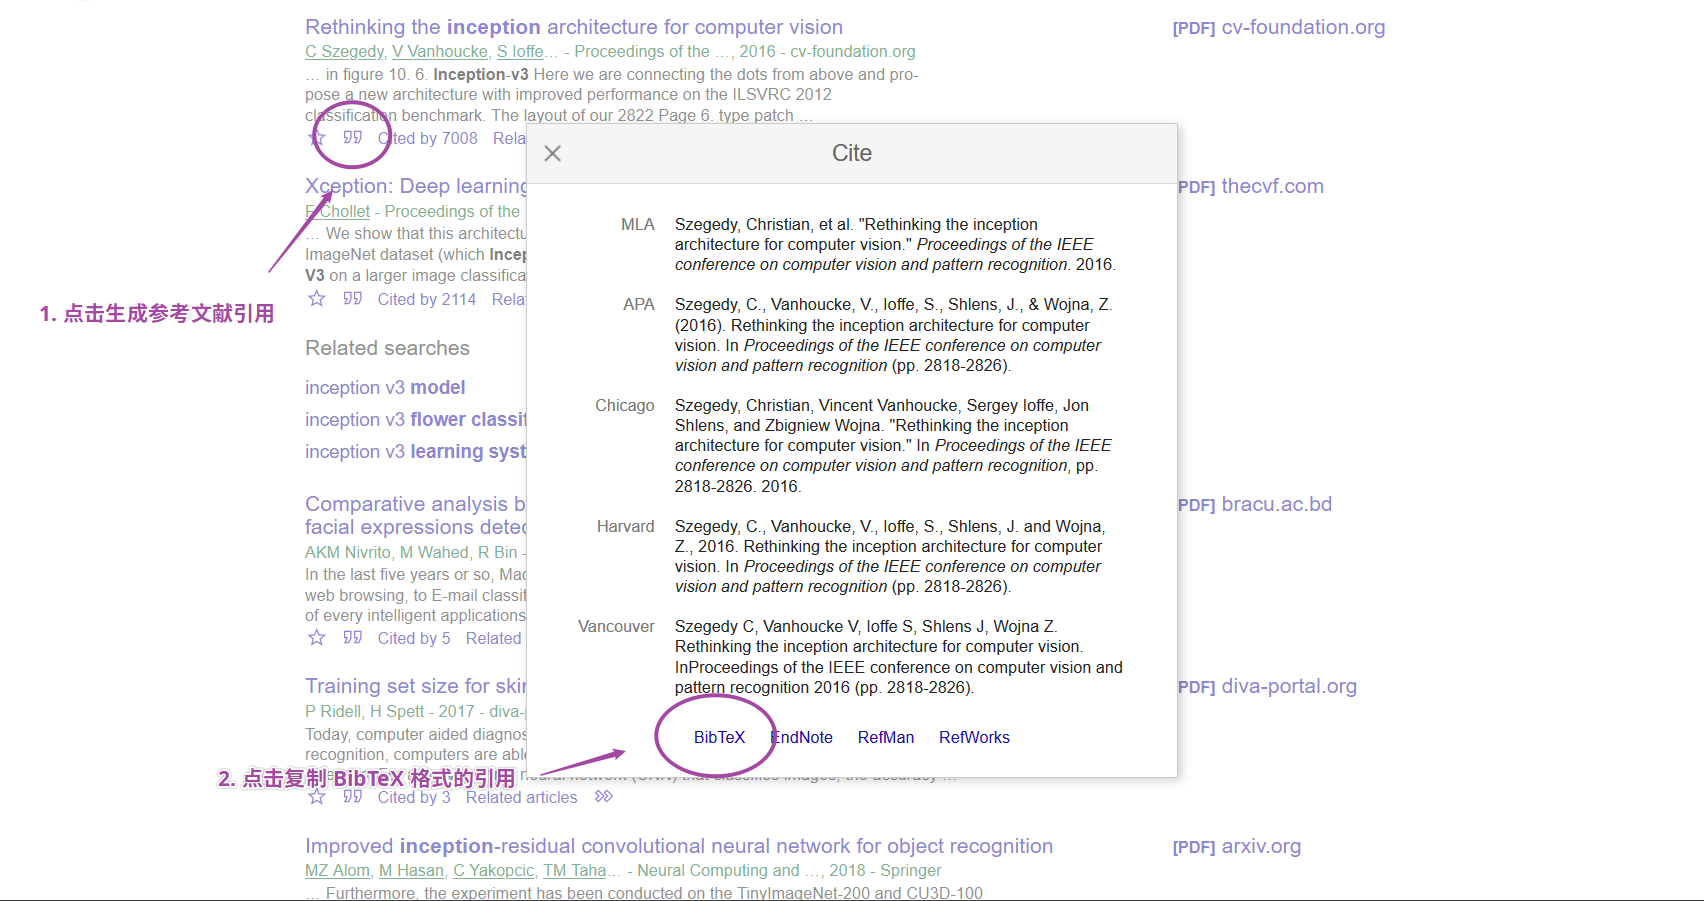
\includegraphics[width=\textwidth]{images/google_scholar.png}
  \caption{谷歌学术搜索并复制文献的 \hologo{BibTeX} 格式}
  \label{google_scholar}
\end{figure}

复制得到的参考文献 \hologo{BibTeX} 类似:

\begin{minted}[frame=single,linenos,breaklines]{tex}
  @inproceedings{szegedy2016rethinking,
    title={Rethinking the inception architecture for computer vision},
    author={Szegedy, Christian and Vanhoucke, Vincent and Ioffe, Sergey and Shlens, Jon and Wojna, Zbigniew},
    booktitle={Proceedings of the IEEE conference on computer vision and pattern recognition},
    pages={2818--2826},
    year={2016}
  }
\end{minted}

将上面的内容复制进入 \texttt{misc/ref.bib} 即可,之后你就可以直接在文章中使用这一参考文献的地方用类似下面的方法引用这一标签为 szegedy2016rethinking 的参考文献:

\begin{minted}[frame=single,linenos,breaklines]{tex}
  正文,正文正文 \cite{szegedy2016rethinking} 正文正文……
\end{minted}

另外,你也可以考虑使用 Zotero 等专业文献管理工具批量生成。参考:\href{https://sspai.com/post/56724}{文献管理神器 Zotero 学习路径指南}。

\begin{figure}[H]
  \center
  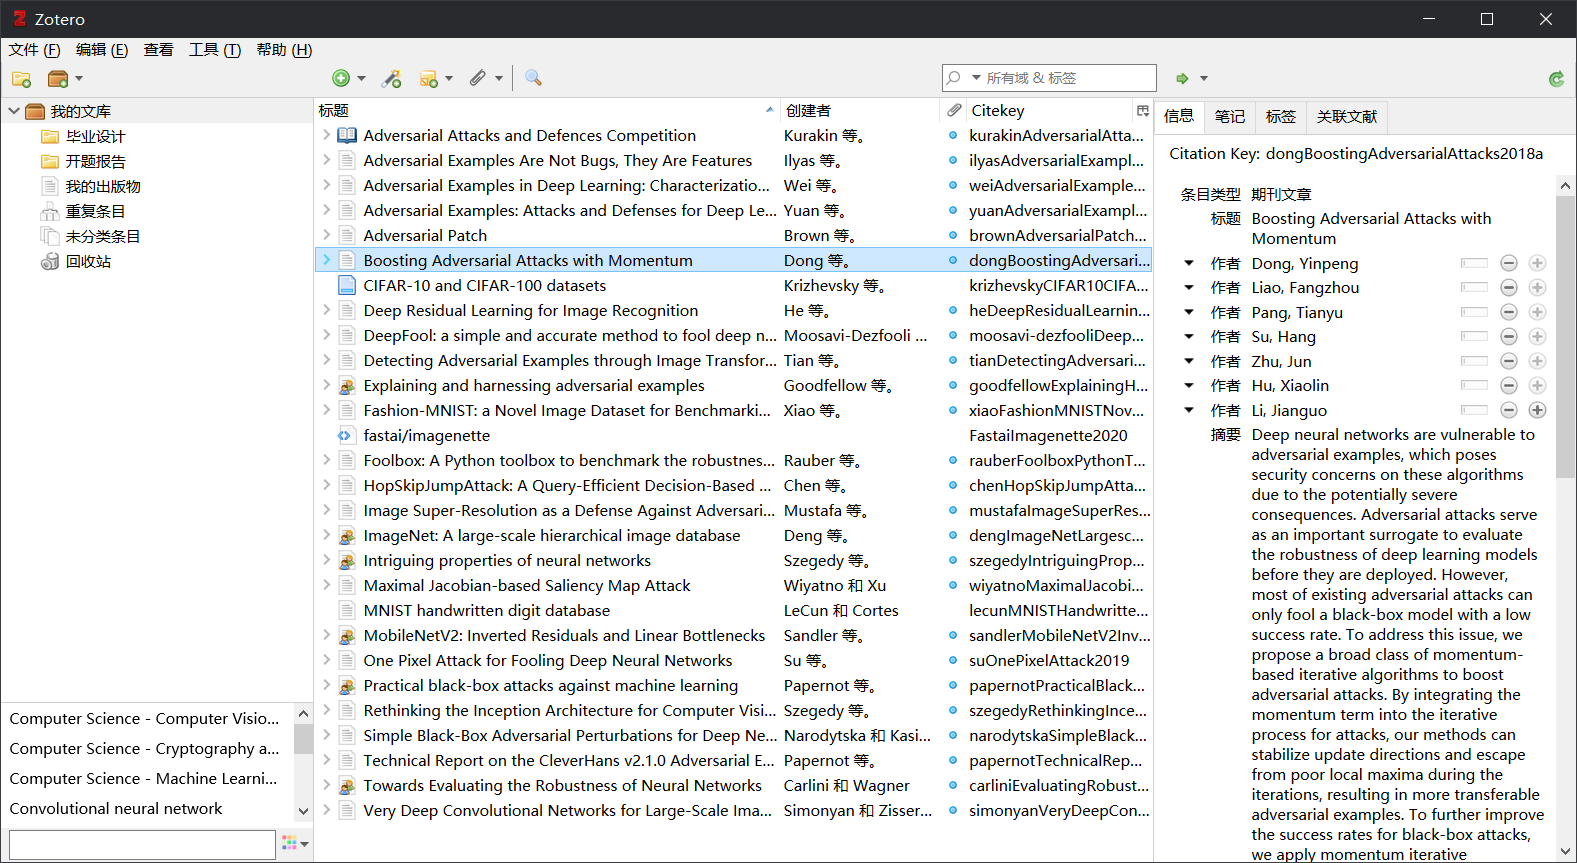
\includegraphics[width=\textwidth]{images/zotero.png}
  \caption{专业文献管理工具 Zotero}
\end{figure}

\subsection{图片素材}

整个模板的图片素材都整理在图片文件夹中:\texttt{./images}。你可以将论文中使用到的图片统一放在这一目录下进行管理,在论文中使用“相对路径”进行引用。你可以用类似下面的语法引用图片:

\begin{minted}[frame=single,linenos,breaklines]{tex}
  \begin{figure}[htbp]
    \vspace{13pt} % 调整图片与上文的垂直距离
    \centering
    
\includegraphics[0.8\textwidth]{images/bit_logo.png}
    \caption{标题序号}
    \label{标题序号} % label 用来在文中索引
  \end{figure}
\end{minted}

可以看到:

\begin{itemize}
  \item 我们首先将图片放置在了一个 \verb|\begin{figure} ... \end{figure}| 的环境中,其中 \texttt{[htbp]} 是用于定位图片。
  \item 之后,在环境中,我们首先使用 \verb|\centering| 保证图片水平居中
  \item 之后用 \verb|\includegraphics[图片大小]{图片路径}| 的格式引用了图片本身
  \item 最后我们定义了图片的说明文字 \verb|\caption{图片说明}| 和图片的标签编号 \verb|\label{图片编号}|,前者显示在图片下方起到说明注释的作用,后者让我们可以用 \verb|\ref{图片编号}| 的语法来在正文中引用图片
\end{itemize}

请注意,为了保证图片引用的格式和 Word 模板完全一致,我们手动设置了 \verb|\vspace{13pt}| 的垂直空白,你引用新图片时,也需要添加这一垂直空白。

在第一章节 \texttt{chapters/1\_chapter1.tex} 中的 \href{https://github.com/spencerwooo/BIThesis/blob/master/graduation-thesis/chapters/1_chapter1.tex#L38-L43}{第 38 行至第 43 行} 是一个示范。

\subsection{表格插入}

表格一直是 {\LaTeX} 排版系统非常强大又非常不好实现的一个模块,如果你希望方便的插入表格,可以统一使用 \href{https://www.tablesgenerator.com/}{LaTeX Tables Generator} 进行生成,再粘贴进入模板之中。

在第一章节 \texttt{chapters/1\_chapter1.tex} 中的 \href{https://github.com/spencerwooo/BIThesis/blob/master/graduation-thesis/chapters/1_chapter1.tex#L47-L60}{第 47 行至第 60 行} 是一个示范。

\subsection{公式插入}

{\LaTeX} 的行内数学符号和公式等,使用 \verb|\( ... \)| 的语法进行定义。比如类似如下的正文:

\begin{minted}[frame=single,linenos,breaklines]{tex}
  The well known Pythagorean theorem \(x^2 + y^2 = z^2\) was
  proved to be invalid for other exponents.
  Meaning the next equation has no integer solutions:

  \[ x^n + y^n = z^n \]
\end{minted}

即可非常简单的渲染如下的公式效果:

The well known Pythagorean theorem \(x^2 + y^2 = z^2\) was proved to be invalid for other exponents. Meaning the next equation has no integer solutions:

\[ x^n + y^n = z^n \]

另外,行内数学环境也可以用 \verb|$ ... $| 的语法进行定义:

\begin{minted}[frame=single,linenos,breaklines]{tex}
  In physics, the mass-energy equivalence is stated
  by the equation $E=mc^2$, discovered in 1905 by Albert Einstein.
\end{minted}

In physics, the mass-energy equivalence is stated
by the equation $E=mc^2$, discovered in 1905 by Albert Einstein.

复杂的独立模块数学公式可以用如下的语法进行定义:

\begin{minted}[frame=single,linenos,breaklines]{tex}
  \begin{equation}
    LRI=1\ ∕\ \sqrt{1+{\left(\frac{{\mu }_{R}}{{\mu }_{s}}\right)}^{2}{\left(\frac{{\delta }_{R}}{{\delta }_{s}}\right)}^{2}}
  \end{equation}
\end{minted}

\begin{equation}
  LRI=1\ ∕\ \sqrt{1+{\left(\frac{{\mu }_{R}}{{\mu }_{s}}\right)}^{2}{\left(\frac{{\delta }_{R}}{{\delta }_{s}}\right)}^{2}}
\end{equation}

为了保证与 Word 模板中的数学公式要求一致,我们的 {\LaTeX} 模板中的公式默认会进行相应的编号(比如上面的例子)。在第一章节 \texttt{chapters/1\_chapter1.tex} 中的 \href{https://github.com/spencerwooo/BIThesis/blob/master/graduation-thesis/chapters/1_chapter1.tex#L67-L69}{第 67 行至第 69 行} 是一个示范。

\subsection{其他}

以下模块的使用可能需要你手动在 \texttt{main.tex} 的开头用 \verb|\usepackage{ ... }| 的方法引入其他 {\LaTeX} 宏包。

\subsubsection{代码高亮}

你可以使用 \texttt{minted} 宏包来进行代码块的渲染。比如:

\begin{itemize}
  \item 在文档开题引入宏包:
  \begin{minted}[frame=single]{tex}
    \usepackage{minted}
  \end{minted}
  \item 渲染代码块:
  \begin{minted}[frame=single]{tex}
    \begin{minted}{python}
      import numpy as np

      def incmatrix(genl1,genl2):
          m = len(genl1)
          n = len(genl2)
          M = None #to become the incidence matrix
          VT = np.zeros((n*m,1), int)  #dummy variable

          #compute the bitwise xor matrix
          M1 = bitxormatrix(genl1)
          M2 = np.triu(bitxormatrix(genl2),1)
      \end{mintd}
  \end{minted}
\end{itemize}

你就会得到类似下面的渲染效果:

\begin{minted}[frame=single]{python}
import numpy as np

def incmatrix(genl1,genl2):
    m = len(genl1)
    n = len(genl2)
    M = None #to become the incidence matrix
    VT = np.zeros((n*m,1), int)  #dummy variable

    #compute the bitwise xor matrix
    M1 = bitxormatrix(genl1)
    M2 = np.triu(bitxormatrix(genl2),1)
\end{minted}

有关 \texttt{minted} 的更多使用方法,请阅读:\href{https://www.overleaf.com/learn/latex/Code_Highlighting_with_minted}{Code Highlighting with minted。}

如果你在使用 \texttt{minted} 的过程中遇到了任何问题,请阅读:\href{https://github.com/spencerwooo/BIThesis/wiki/Troubleshooting}{疑难杂症 Troubleshooting}。

\subsubsection{算法模块}

你可以使用 algorithm2e 宏包来渲染一个“伪代码算法”模块。比如:

\begin{itemize}
  \item 在文档开头引入宏包:
  \begin{minted}[frame=single]{tex}
    \usepackage[ruled,vlined]{algorithm2e}
  \end{minted}
  \item 渲染伪代码模块:
  \begin{minted}[frame=single]{tex}
    \begin{algorithm}[H]
    \SetAlgoLined
    \KwResult{Write here the result }
      initialization\;
      \While{While condition}{
      instructions\;
      \eIf{condition}{
        instructions1\;
        instructions2\;
        }{
        instructions3\;
        }
      }
    \caption{How to write algorithms}
    \end{algorithm}
  \end{minted}
\end{itemize}

这样,你就会得到类似如下的渲染效果:

\begin{algorithm}[H]
  \SetAlgoLined
  \KwResult{Write here the result }
  initialization\;
  \While{While condition}{
  instructions\;
  \eIf{condition}{
    instructions1\;
    instructions2\;
    }{
    instructions3\;
    }
  }
  \caption{How to write algorithms}
\end{algorithm}

有关更多伪代码算法模块的使用,请阅读:\href{https://www.overleaf.com/learn/latex/algorithms}{Algorithms}。

\clearpage
\section{通用北京理工大学本科生实验报告模板使用指南} \label{lab-report}

\tipbox{说明:这个实验报告模板是一个通用的报告模板,不适用所有实验报告要求。实验课程未提供实验报告模板时可以使用该模板。当前本实验报告模板只包含一个封面,欢迎大家往项目仓库 PR 制作更多的封面。}

\subsection{熟悉项目}
\dirtree{%
  .1 /.
  .2 README.md.
  .2 main.pdf.
  .2 main.tex.
  .2 misc.
  .3 cover\_v1.tex.
  .2 assets.
  .3 …….
}

\begin{itemize}
  \item[\color{RubineRed}\textbf{\texttt{main.tex}}] tex 源文件,本实验报告模板的主体文件,所有需要添加的内容都在该文件里进行修改即可
  \item[\color{RubineRed}\textbf{\texttt{main.pdf}}] 编译项目生成的 pdf 文件
  \item[\color{RubineRed}\textbf{\texttt{./misc}}] 杂项(包括实验报告封面等):
        \begin{itemize}
          \item[\color{RoyalBlue}\texttt{cover\_v1.tex}] 这是一个示范性的报告封面,该文件无需修改
        \end{itemize}
  \item[\color{RubineRed}\textbf{\texttt{./asset}}] 一些图片资源存放文件夹
\end{itemize}

\subsection{编译方式与使用}

由于实验报告模板没有涉及到参考文献的使用,因此我们只需要使用 \hologo{XeLaTeX} 即可进行全文编译。

整个项目的编译工具链的顺序为:
\begin{center}
  \begin{tikzpicture}[
      bib/.style={rectangle, draw=ForestGreen!60, fill=ForestGreen!5, very thick, minimum size=8mm},
      xe/.style={rectangle, draw=RubineRed!60, fill=RubineRed!5, very thick, minimum size=8mm},
    ]
    % Nodes
    \node[xe] (xelatex1) {xelatex};
    \node[xe] (xelatex2) [right=of xelatex1] {xelatex};
    \node[xe] (xelatex3) [right=of xelatex2] {xelatex};

    % Arrows
    \draw[->] (xelatex1.east) -- (xelatex2.west);
    \draw[->] (xelatex2.east) -- (xelatex3.west);
  \end{tikzpicture}
\end{center}

其中,按照 VS Code 的 LaTeX Workshop 设置格式:{\hologo{XeLaTeX}} 的编译命令为:

\begin{minted}[frame=single]{json}
  {
    "name": "xelatex",
    "command": "xelatex",
    "args": [
      "-synctex=1",
      "-interaction=nonstopmode",
      "-file-line-error",
      "-pdf",
      "-outdir=%OUTDIR%",
      "-cd",
      "%DOC%"
    ],
    "env": {}
  }
\end{minted}

整个编译的 recipe 为:

\begin{minted}[frame=single]{json}
  {
    "name": "xelatex * 3",
    "tools": [
        "xelatex",
        "xelatex",
        "xelatex"
    ]
  }
\end{minted}

\paragraph{使用}

各种内容的插入请参考源文件。

\clearpage
\section{如何将 {\LaTeX} 文档转换为 Word}

如果你决定使用 {\LaTeX} 进行论文撰写,但是你的导师希望你提供 Word 版本的论文进行方便的批注等,你可以使用下面的方法来将你的 {\LaTeX} 论文转换为 Word 格式的文档。需要注意的是,这种方式的转换并不能完整的将 {\LaTeX} 论文的全部格式进行转换,仅能保证正文部分内容的不丢失,其余包括“论文封面”、“表格”等等部分的内容,在转换的过程中都可能丢失。这些部分需要你后期手动进行添加。

\subsection{安装 Pandoc 命令行工具}

Pandoc 是一个支持几乎所有 Markup 格式文档的“通用文档转换器”,是一个命令行工具,支持所有常用操作系统。我们可以借助 pandoc 进行格式转换。

Pandoc 详细的安装说明请见官方文档:\href{https://pandoc.org/installing.html}{Installing pandoc}.

简单来说:

\begin{itemize}
  \item 在 Windows 上你可以使用 scoop 包管理工具安装 pandoc(为了方便设置命令行工具的环境变量,推荐使用 scoop 进行安装):
  \begin{minted}[frame=single]{bash}
  scoop install pandoc
  \end{minted}
  \textbf{关联阅读:}\href{https://sspai.com/post/52496}{“一行代码”搞定软件安装卸载,用 Scoop 管理你的 Windows 软件}
  \item 在 macOS 上你可以使用 Homebrew 包管理工具安装 pandoc:
  \begin{minted}[frame=single]{bash}
  brew install pandoc
  \end{minted}
  \item 在 Linux 上你可以使用你所用发行版的包管理工具安装 pandoc,比如:
  \begin{minted}[frame=single]{bash}
  sudo apt install pandoc
  \end{minted}
\end{itemize}

之后,在终端中输入:
\begin{minted}[frame=single]{bash}
  pandoc --version
\end{minted}

如果出现类似下面的输出,说明你的 pandoc 安装成功。

\begin{figure}[H]
  \centering
  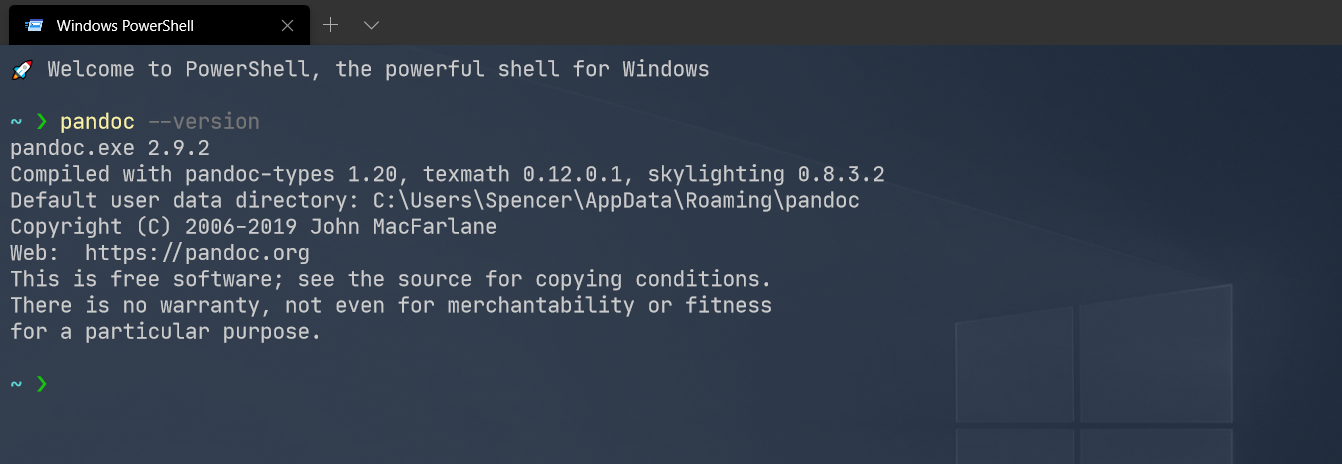
\includegraphics[width=\textwidth]{images/pandoc_test.png}
  \caption{测试 pandoc 安装成功}
  \label{pandoc_test}
\end{figure}

\subsection{完善 Word 格式的模板文件}

为了保证导出的 Word 文档格式和学校提供的模板大体一致,我们需要确认 Word 版本的模板\textbf{已经准确定义了各级标题、正文等部分的格式。}

\begin{figure}[H]
  \center
  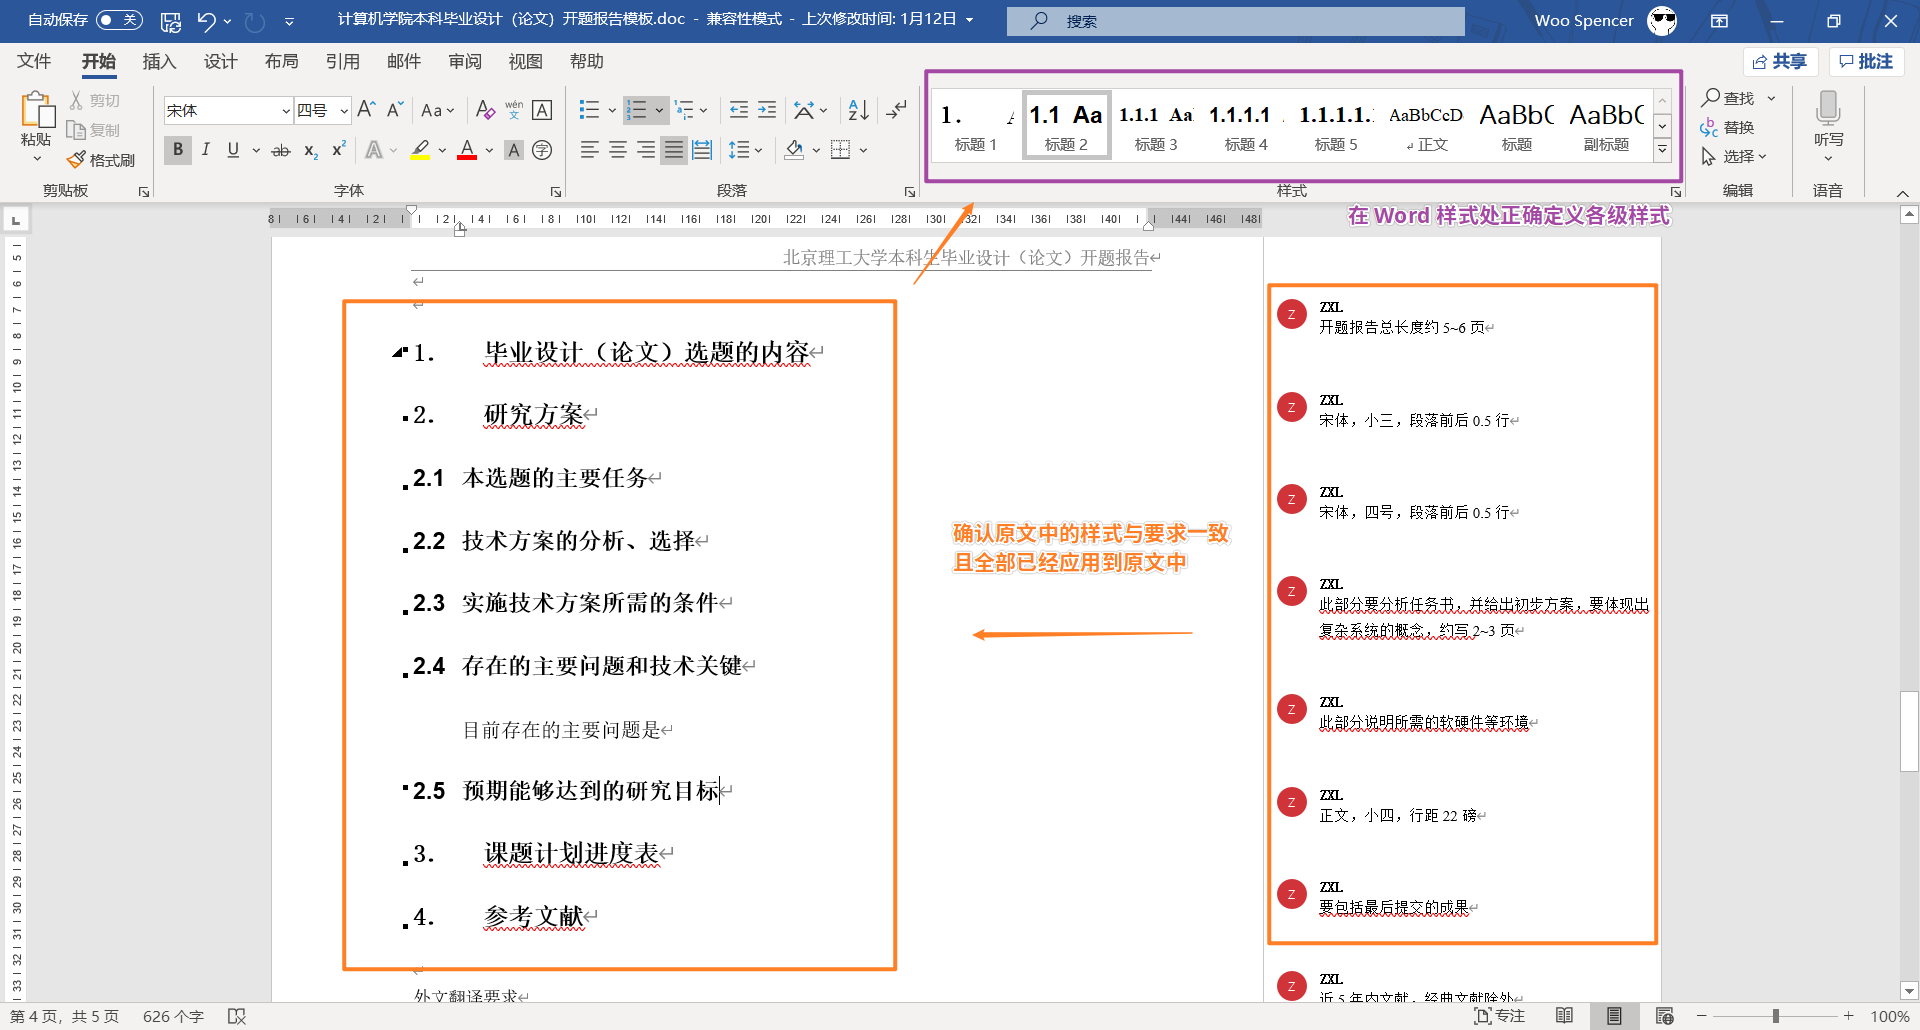
\includegraphics[width=\textwidth]{images/latex_pandoc_word.png}
  \caption{确认 Word 版本的模板准确生成}
  \label{latex_pandoc_word}
\end{figure}

之后,我们需要将这一文件(\texttt{doc} 或 \texttt{docx})保存,\textbf{留作 pandoc 的格式参考。}

\subsection{进行格式转换}

最后,我们进行格式的转换。

\subsubsection{朴素格式转换}

如果你只希望将文本内容导出为 Word,不在意格式或其他内容的正确性,你可以直接使用下面的命令进行最普通的文本转换:

\begin{minted}[frame=single]{bash}
  pandoc {LaTeX 文档文件} -o {输出 Word 文档}
\end{minted}

比如:

\begin{minted}[frame=single]{bash}
  pandoc main.tex -o main.docx
\end{minted}

没有特别指明模板 Word 文档格式与参考文献文档的情况下,pandoc 仅会处理你 {\LaTeX} 文档中的文字内容,按照标题、正文的格式整理进入 Word。

\subsubsection{含有目标模板 Word 文档的格式转换}

如果你希望按照模板 Word 文档的规定格式进行转换,那么你可以直接使用下面的命令进行格式转换:

\begin{minted}[frame=single,linenos,breaklines]{bash}
  pandoc {LaTeX 文档文件} --reference-doc={参考模板 Word 文档} -o {输出 Word 文档}
\end{minted}

比如,我们的 {\LaTeX} 文档文件名称为 \texttt{main.tex},参考模板 Word 文档名称为 \texttt{template.docx},希望输出名为 \texttt{main.docx} 的 Word 文档,我们即可如下组织 pandoc 转换命令:

\begin{minted}[frame=single]{bash}
  pandoc main.tex --reference-doc=template.docx -o main.docx
\end{minted}

\subsubsection{含有参考文献文档的格式转换}

如果你的 LaTeX 文档中包含有参考文献的引用,那么你需要特别明确参考文献 \hologo{BibTeX} 文件,将文件以 \texttt{--bibliography=\{参考文献文件\}} 的参数告知 pandoc,从而让 pandoc 正确处理你的参考文献。比如:

\begin{minted}[frame=single,linenos,breaklines]{bash}
  pandoc main.tex --bibliography=refs.bib --reference-doc=template.docx -o main.docx
\end{minted}

特别强调:pandoc 格式转换功能有限,无法处理 {\LaTeX} 多级嵌套表格(在本模板的“开题报告”与“毕业论文”中都有使用多级嵌套表格,直接调用 pandoc 默认情况下会报错。需要删掉 {\LaTeX} 文档中的表格,并后期手动录入 Word 之中),也无法保证格式与 {\LaTeX} 原文档 \textbf{完全一致},都需要我们后期手动进行调整。

\clearpage
\section{疑难杂症}

\clearpage
\section{致谢}

{\BIThesis} 模板是一个团队项目。从一个开题报告的启发,到最终完成程度接近 100\%,格式几乎完全匹配的毕业论文;从一个简陋的 README,到近一万两千字的在线版本 Wiki 文档和近一万字的 {\LaTeX} PDF 文档(本文档)……这些离不开团队成员(2016 级计算机学院本科生武上博、2016 级计算机学院本科生王赞)两位同学近一个月的努力与维护,他们见证了 {\BIThesis} 的从无到有。

作为 {\BIThesis} 的创造者,我(武上博)由衷的感谢北京理工大学教务部、北京理工大学计算机学院教务处为我们项目提供的强大背书,没有支持我们的领导和老师们的助力,本项目将毫无意义;感谢最初打开、阅读、与分享这一项目的介绍公众号文章的各位老师与同学,没有愿意分享这一项目的你们,本项目将无人问津;感谢愿意为这一项目在 GitHub 上做出贡献、提出 pull request 的诸位同学,没有你们的贡献,本项目也不会有这么多的特色;感谢因为各种问题在 GitHub 的 issue 上进行询问的同学,没有你们的提问,本项目同样也不会这样完善。当然,最终,也要感谢使用 {\BIThesis} 的同学们,你们为我们的工作赋予了意义,为我们的后续维护提供了动力,感谢你们,感谢所有人。

本文档是 {\BIThesis} 的官方参考手册,由 2016 级计算机学院武上博同学、2016 级计算机学院王赞同学撰写,感谢 2016 级计算机学院唐誉铭同学、2017 级经济与管理学院詹熠莎同学提供的宝贵意见。


\end{document}
